%%%%%%%%%%%%%%%%%%%%%%%%%%%%%%%%%%%%%%%%%%%%%%%%%%%%%%
% Esse template foi um fork do 
% https://github.com/lucasmsoares96/Template-Monografia-CEFET-MG
% Modificado para atender aos padrões da FACE-UFMG
% Já está usando as atualizações da abnt de 2023 para as citações
% Esse documento é dividido em três arquivos tex diferentes: pre_textual.tex, textual.tex e pos_textual.tex
%
%%%%%%%%%%%%%%%%%%%%%%%%%%%%%%%%%%%%%%%%%%%%%%%%%%%%%%

\documentclass[a4paper,12pt,oneside]{memoir}
\usepackage[utf8]{inputenc}
\usepackage{FACE}
\usepackage{lipsum}    % gera texto aleatório (remover)
% Ramon:
\usepackage{amsmath}
\usepackage{amssymb}
\usepackage{booktabs}
\usepackage{adjustbox}
\usepackage{tabularx}
\usepackage{caption} % Para usar \captionof
\usepackage{array}
\usepackage{float}
\usepackage{algorithm}
\usepackage{algpseudocode}
\usepackage{color} % for text color
\usepackage{colortbl} % for table colors
\usepackage[table,xcdraw]{xcolor} % for more color options
\usepackage{soul} % for strikethrough text
\usepackage{booktabs} % for table rules
\usepackage{setspace} % for line spacing
\usepackage{pdflscape} % Pacote para orientação paisagem
%\usepackage{placeins} % Para \FloatBarrier
\usepackage{afterpage} % Para controlar a página seguinte
\usepackage{rotating}
\usepackage{xurl}
\interfootnotelinepenalty=10000 % for url to not break across pages


%%%%%%%%%%%%%%%%%%%%%%%%%%%%%%%%%%%%%
%                                   %
% Incluir o arquivo de bibliografia %
%                                   %
%%%%%%%%%%%%%%%%%%%%%%%%%%%%%%%%%%%%%
\addbibresource{bibliografia.bib}


% Configurações do Documento
\title{O papel das convenções na política monetária:}
\subtitle{interlocuções entre a teoria pós-keynesiana e avanços recentes da linguística computacional}
\author{Ramon da Silva Torres}  

\date{2024}
\location{Belo Horizonte}


\advisor{Orientador: Rafael Saulo Marques Ribeiro}
\coadvisor{Coorientador: Marco Flávio da Cunha Resende}

\committeeone{Membro da Banca 1\\ Título}
\committeetwo{Membro da Banca 2\\ Título}
% \committeethree{Título Nome\\ Titulação} Se houver terceiro membro da banca modificar também o arquivo FACE.sty


% Lembre de colocar a data real no lugar de "\today" antes de imprimir a folha de aprovação
\committeedate{\_\_\_\_\_\_\_\_\_\_\_\_}

\institution{
  Universidade Federal de Minas Gerais
  \\
  Faculdade de Ciências Econômicas
  \\
  Departamento de Ciências Econômicas
}

\preamble{Projeto de Qualificação apresentado ao Departamento de Ciências Econômicas da Universidade Federal de Minas Gerais, como requisito parcial à obtenção do título de Doutor em Ciências Econômicas.}


\begin{document}
\selectlanguage{brazil}
\frontmatter
\pretextual
\maketitle
%\makecover % folha de rosto               (obrigatório)
% Se houver errata, deverá ser incluída após a folha de rosto

% ---
% Após a apresentação do trabalho incluir o pdf com a folha com as assinaturas utilizando os seguintes comandos.
% 
% \begin{titlingpage*}
% \includepdf{folha_assinada.pdf}
% \end{titlingpage*}
%
%\makeapproval %  (obrigatório)

%\dedication{Folha na qual o autor presta uma homenagem ou dedica seu trabalho. Não leva título e a dedicatória deve aparecer na parte inferior da página, a 8cm da margem esquerda.}

%\clearpage\pagestyle{empty}
%\chapter*{Agradecimentos}
%"Expressos pelo autor que presta seu reconhecimento às pessoas e instituições que
%colaboraram na elaboração do seu trabalho. Não leva indicativo numérico e o título
%deve ser centralizado na folha, utilizando a mesma tipologia das seções primárias do
%texto." conforme o manual de normalização página 10.
%\clearpage

% \input{1-Pre-Textual/Epigrafe.tex}%       (opcional)

%\epigraph{only a boring man will always want things to match;
%real quality lies in irregularity}{Yoshida Kenkō}

%\clearpage\pagestyle{empty}
% \input{1-Pre-Textual/Resumo.tex} %        (obrigatório)

%\begin{abstract}
%    É a apresentação concisa dos pontos relevantes do texto, fornecendo uma visão rápida
%    e clara do conteúdo do trabalho e das conclusões alcançadas, de tal forma que este
%    possa dispensar a consulta ao original. Deve ter uma extensão de 150 a 500 palavras.
%    Abaixo do resumo devem figurar as palavras-chave, representativas do conteúdo do
%    trabalho. Devem ser precedidas da expressão Palavras-chave: separadas entre si por
%    ponto e finalizadas também por ponto.
%    \\ \\
%    \textbf{Palavras-chave:} Palavra-chave 1; Palavra-chave 2; Palavra-chave 3; Palavra-chave 4; Palavra-chave 5.
%\end{abstract}
%\clearpage

% \input{1-Pre-Textual/Abstract.tex} % 
%\begin{otherlanguage}{brazil}
%    \begin{abstract}
%        Tradução do resumo em língua vernácula preferencialmente para o inglês. Deve ser
%        seguido das palavras-chave traduzidas para a mesma língua.
%        Localizado logo após o resumo em língua vernácula.
%        \\ \\
%        \textbf{Keywords:} Keywords 1; Keywords 2; Keywords 3; Keywords 4; Keywords 5.
%    \end{abstract}
% \end{otherlanguage}
%\clearpage


%\listoffigures* %                          (opcional)
% \listoftables*  %                          (opcional)


% --- Lista de abreviaturas (opcional)
% Lista de abreviaturas usando o pacote acronym. As abreviaturas precisam ser usadas no texto usando o comando \ac{} na primeira vez que for invocado ele substituirá a descrição longa e nas vezes subsequentes incluirá apenas a sigla com um link para a definição na lista de abreviaturas 
% ---

% \chapter*{Lista de Abreviaturas e Siglas}
% \begin{acronym}
%     \acro{API}{Interface de Programação de Aplicativos, do inglês \textit{Application Programming Interface}}
%     \acro{CPU}{Unidade Central de Processamento, do inglês \textit{Central Processing Unit}}
%     \acro{DAG}{Grafos Acíclicos Dirigidos, do inglês \textit{Directed Acyclic Graph}}
%     \acro{GC}{Coletor de Lixo, do inglês \textit{Garbage Collector}}
%     \acro{VM}{Maquina Virtual, do inglês \textit{Virtual Machine}}
% \end{acronym}


% ---
% inserir lista de símbolos
% ---
% \nomenclature{$\alpha$}{Letra grega minúscula alpha}
% \nomenclature{$\rightarrow$}{"Tem seu valor alterado para..."}
% \nomenclature{$\propto$}{"é proporcional à..."}
% \nomenclature{$\lesssim$}{"Aproximadamente menor que..."}
% \nomenclature{$\gg$}{"Muito maior que..."}
% \printnomenclature

% \clearpage

\tableofcontents* %                        (obrigatório)

\mainmatter
\textual
\chapterstyle{texto}
\chapter{Projeto de Qualificação} \label{projeto}
% ----------------------------------------------------------

\section{Introdução}


O Dicionário Brasileiro da Língua Portuguesa \textit{Michaelis} define a palavra \enquote{Convenção} como \enquote{Acordo, ajuste ou combinação sobre determinado assunto [...]}\footnote{https://michaelis.uol.com.br/moderno-portugues/busca/portugues-brasileiro/conven\%C3\%A7\%C3\%A3o/}. O Dicionário de \textit{Cambridge} para a Língua Inglesa define \enquote{\textit{Convention}} como \enquote{\textit{a usual or accepted way of behaving [...] often following an old way of thinking or a custom [...]}}\footnote{https://dictionary.cambridge.org/pt/dicionario/ingles/convention}. Ambas as definições antecipam parcialmente o significado que o termo irá assumir ao longo deste trabalho: uma crença compartilhada entre os indivíduos sobre o estado da economia. 

Essa acepção está atrelada ao arcabouço teórico pós-keynesiano, no qual o conceito de convenção é resgatado da \textit{Teoria Geral} para compor o quadro dos elementos que guiam o comportamento dos agentes econômicos em um ambiente de incerteza fundamental \textcite{carvalho_keynes_2020}. A pedra angular dessa teoria, como se verá, é a incerteza fundamental quanto ao futuro. Se se admite que o futuro pode não repetir o passado - no que se refere às propriedades estatísticas das séries de dados (média, variância, autocorrelação, dentre outras) - então o conhecimento probabilístico não pode ser obtido para servir como guia de conduta para a tomada de decisões. Os agentes se voltam então a estratégias defensivas como forma de atenuar o problema da incerteza. No plano institucional, os contratos a termo se destacam enquanto uma forma de impor uma rigidez ao futuro, enquanto trazem previsibilidade para o presente. No plano cognitivo, são as convenções que estruturam as regras de pensamento e comportamento dos agentes, possibilitando alguma forma de coordenação em um ambiente incerto \parencite{abramo_cidade_2007, erber_as_2011, carvalho_keynes_2020, dequech_conventions_2022}.



A temática das convenções, contudo, não ocupou lugar de destaque entre os pós-keynesianos. Poucos títulos de trabalhos, seções ou capítulos carregam o termo. Apenas para \enquote{\textit{some schollars}} a noção de convenção ocupa um lugar central na teoria de Keynes \parencite[p. 145]{dequech_conventions_2022}. É possível que isso se deva ao fato de que o próprio Keynes, ao oferecer o conceito de comportamento convencional no capítulo 12 da \textit{Teoria Geral}, estava mais interessado em extrair seus efeitos do que explorar o conceito em si \parencite[p. 238]{carvalho_keynes_2020}. Uma teoria das convenções permaneceu assim, em aberto, ofuscada por outros conceitos que, no plano cognitivo-comportamental dos agentes ante a incerteza, carregaram maior atenção: a preferência pela liquidez, o comportamento de manada e o \enquote{\textit{animal spirit}}\footnote{Embora o comportamento de manada possa ter como base uma convenção, a literatura costuma enfatizar a ausência de ‘expectativas racionais’ nesse comportamento e seu potencial para amplificar as oscilações das variáveis econômicas, sem, contudo, debater o conceito de convenção e seu papel para o comportamento de manada}.

Este trabalho procura resgatar a noção de convenção em Keynes e entre os pós-keynesianos, conferindo-a tratamento empírico. Busca-se debater a capacidade do conceito de contribuir para a discussão moderna de política monetária, na qual a comunicação entre bancos centrais e mercado tem sido alçada à posição de instrumento próprio de política monetária \parencite{blinder_central_2008}. A convenção no plano teórico e a comunicação no plano empírico compõem as duas dimensões do problema que se busca analisar neste trabalho.  

A seguinte passagem, extraída da \textit{Teoria Geral}, apresenta o ponto de partida desta pesquisa.  

\begin{quote}
\footnotesize % Diminui o tamanho da letra
\setlength{\leftskip}{2cm} 
\enquote{A taxa de juros de longo prazo dependerá não apenas da política corrente da autoridade monetária, mas também das \textbf{expectativas} do mercado no que se refere a sua política futura. A autoridade monetária controla com facilidade a taxa de juros de curto prazo ... Mas a taxa de longo prazo pode mostrar-se mais recalcitrante quando cai a um nível que, com base na experiência passada e nas expectativas correntes da política monetária futura, a \textbf{opinião abalizada} considera inseguro ... uma política monetária que atinge a \textbf{opinião pública} como sendo de caráter experimental ou facilmente alterável pode falhar [...] A mesma política [...] pode se provar facilmente bem-sucedida se ela aparece à \textbf{opinião pública} como razoável e praticável ... Talvez seja mais exato dizer que a taxa de juros é um fenômeno \textbf{convencional}, ao invés de psicológico, pois o seu valor observado depende sobremaneira do valor futuro que se lhe prevê. Qualquer taxa de juros \textbf{aceita com suficiente convicção} como provavelmente duradoura será duradoura; sujeita, naturalmente, em uma sociedade em mudança, a flutuações, originadas por diversos motivos, em torno do nível normal esperado.} \parencite[p. 203, grifos do autor]{keynes_teoria_1996}
\end{quote}

Se se pode dizer, conforme a passagem, que a convenção está associada à opinião, seria possível mensurá-la? Seria possível acessar a convenção, relacionando-a com as demais variáveis macroeconômicas, investigando a significância de seu efeito? 

Essas perguntas levaram esta pesquisa a adentrar na área da Linguística Computacional, onde foi possível aplicar o ferramental metodológico capaz de extrair as opiniões e sentimentos dos indivíduos por meio de fontes textuais. Esse ferramental tem sido extensivamente utilizado para com dados de redes sociais em anos recentes \parencite{carosia_analyzing_2020, garcia_topic_2021, de_melo_comparing_2021, de_carvalho_mining_2022}. Estes espaços virtuais, amplamente difundidos entre a população, servem como meio de se posicionar politicamente, culturalmente e economicamente. A importância das redes sociais enquanto \textit{locus} de obtenção de informação pelos agentes econômicos tem sido destacado por alguns estudos \parencite{carosia_analyzing_2020, paiva_essays_2022}. Em geral, dias em que os serviços de redes sociais foram interrompidos levaram a queda na quantidade de investidores e no volume negociado \parencite{paiva_essays_2022}.

Escolheu-se a rede social X (anteriormente \textit{Twitter}), como fonte primária de informação, por ser uma rede social com predomínio da linguagem textual.
A base de dados foi obtida através de um algoritmo de mineração de dados (\textit{webscraping}) construído na linguagem de programação \textit{Python} pelo autor do presente projeto. Ao todo, foram coletadas 55.129.584 postagens em português com temáticas econômicas realizadas entre 2008 e 2022. Destas, 5.066.044 se referem à política monetária.

Este trabalho procura explorar esses dados textuais de forma a extrair um indicador de sentimento a respeito da política monetária. Busca-se investigar a capacidade de esse indicador representar a convenção sobre a política monetária, ou seja, o posicionamento entre os agentes sobre os rumos adotados pela autoridade monetária. Resgatando as definições acima, seria o indicador uma medida do nível de \enquote{acordo} ou de \enquote{combinação} entre agentes de mercado e Banco Central a respeito da política monetária?

O passo seguinte à construção do indicador é sua utilização em modelos de séries temporais de forma a testar sua significância ante à outras variáveis macroeconômicas. Nesse sentido, modelos do tipo VAR tem sido a principal opção metodológica empregada pela literatura \parencite{bloom_impact_2009, lucca_measuring_2009, haddow_macroeconomic_2013, baker_measuring_2016, nyman_news_2021}. Em comum, todos estes trabalhos constroem índices de sentimento com base em informações textuais (noticiários, redes sociais, comunicados dos bancos centrais) e averíguam seu impacto em variáveis macroeconômicas, particularmente os juros de longo prazo. 

É este o empreendimento deste trabalho. Parte-se da teoria pós-keynesiana, em especial da noção de convenção, para esboçar uma estrutura teórica de formação das taxas de juros no longo prazo. Investiga-se a literatura que trabalha de forma empírica o papel da comunicação do Banco Central na política monetária. Adentra-se na área da Linguística Computacional como forma de transformar um dado textual em uma informação numérica (indicador), passível de ser utilizado em modelagens quantitativas. Posteriormente, esse indicador é utilizado em modelos de séries temporais, tais como modelos VAR e \textit{Local Projections}, para investigar sua relação com variáveis macroeconômicas, em especial as taxas de juros de longo prazo, por carregarem um elevado componente \enquote{convencional} em sua determinação. 

\clearpage



\section{Justificativa}

O papel da convenção dentro do arcabouço teórico pós-keynesiano é tema controverso. O ponto de atrito entre os autores está na possibilidade de o conceito ser utilizado fora do âmbito do mercado financeiro, onde foi explicitamente empregado por Keynes \parencite{dequech_conventions_2022}. A questão central é se o conceito poderia ser estendido do mercado financeiro, da compra de ativos líquidos, para o mercado de bens, especificamente, os bens de capital, por sua vez ilíquidos, contribuindo, assim, para a teoria de determinação do investimento. Segundo \textcite{dequech_conventions_2022}, entre os autores que advogam pela restrição do conceito estão \textcite{possas_racionalidade_2016} e \textcite{carvalho_keynes_2020}. Entre os que apelam para seu uso mais generalizado, influenciando inclusive o investimento, estão \textcite{odonnell_keynes_1991}, \textcite{meeks_keynes_2003}, \textcite{dow_keynes_2013}.  

Segundo \textcite[p. 160]{carvalho_keynes_2020}, o conceito de convenção não embasa uma teoria das expectativas de longo prazo e, portanto, não pode servir como elemento definidor do investimento em bens de capital fixo. Nesse sentido, o comportamento convencional, tal como esboçado por 
\textcite{keynes_general_1937, keynes_teoria_1996}, estaria restrito às expectativas de curto prazo, particularmente aquelas relacionadas ao mercado financeiro, podendo ser útil para investigar o comportamento de preços de ações, por exemplo
\footnote{Não obstante, \textcite[Cap. 5]{keynes_teoria_1996} também trata de expectativas de curto prazo não embasadas pelo comportamento convencional, ligadas ao processo de produção. Conforme \textcite{carvalho_expectativas_2014}, para Keynes, as expectativas associadas à produção são de curto prazo e adaptativas.}.

Neste momento, é conveniente esclarecer o mecanismo pelo qual as convenções poderiam afetar algumas variáveis econômicas, em particular as taxas de juros e o nível de investimento. 

Na teorização pós-keynesiana, as decisões de investimento ocorrem em um ambiente permeado pela incerteza fundamental. Essa incerteza se diferencia do risco probabilístico porque o agente não consegue alcançar uma distribuição de probabilidade que seja única, aditiva e confiável sobre um evento futuro, uma vez que informações necessárias tal só serão reveladas no futuro \parencite{dequech_uncertainty_2011}. Isto é, as informações seriam sempre incompletas no momento da tomada de decisão, impedindo o cálculo atuarial. Diante desse cenário, os agentes econômicos adotam certos comportamentos defensivos ante a incerteza, tal como a preferência pela liquidez e a adoção de contratos a termo. Esses comportamentos atenuam o problema da incerteza, mas não o eliminam. Os investimentos ainda podem falhar. Perdas irreversíveis podem ocorrer. Ainda assim, mesmo neste cenário sombrio sob o qual pairam os investimentos sob a incerteza, constata-se que o processo de acumulação capitalista é inegável. Então, pode-se dizer que a força da ação empreendedora ante o incerto é maior do que a força paralisadora da incerteza. 

O que sustenta essa força de ação empreendedora? Na esfera do indivíduo, poder-se-ia dizer que este é dotado de um \enquote{espírito animal}, ávido pelo lucro monetário e pela acumulação \parencite{abramo_cidade_2007}. Mas a força apenas da iniciativa individual do empresário capitalista é limitada ante o destino incerto. Muitos empresários tomam decisões de produção e investimento simultaneamente, não existindo uma coordenação prévia dos planos de produção - este é um dos princípios de uma economia monetária de produção, segundo \textcite{carvalho_keynes_2020}. O futuro com o qual os empresários poderão avaliar suas decisões de investimento e produção será o produto de todas essas decisões simultâneas e conjuntas. Eis que a convenção surge, na esfera coletiva, como uma possibilidade de coordenação entre os agentes \parencite{abramo_cidade_2007, carvalho_expectativas_2014}. 

Sendo essencialmente uma crença compartilhada, a convenção aponta o que a coletividade pode esperar do futuro. Empreendendo ações em torno de um futuro \enquote{acordado}, a convenção carrega em si um caráter profético, assemelhando-se às expectativas autorrealizáveis. O sucesso da materialização da convenção depende, contudo, de sua adesão pelos agentes. Quanto mais agentes se comportarem esperando uma determinada taxa de juros de longo prazo, ou um determinado nível de investimento, maior a chance daquilo que se espera realizar. 

A convenção não é a única forma possível de coordenação. Keynes destacou sobretudo o papel das instituições e da política econômica do Estado - não obstante, as próprias políticas públicas coordenam as expectativas por meio da sua influência sobre as convenções \parencite{resende_ciclo_2020}. O destaque, entre Keynes e os pós-keynesianos, recai sobre a política fiscal, capaz de reduzir incertezas quanto ao futuro ao sinalizar a estabilização da demanda agregada via políticas anticíclicas. Este compromisso do Estado ante ao futuro poderia gerar informações passíveis de serem utilizadas nos cálculos empresariais \textcite[p. 157]{carvalho_keynes_2020}. Contudo, ressalta-se, as instituições e a política econômica são instrumentos de coordenação não mercantis, enquanto a convenção emerge de um acordo tácito no âmbito empresarial \parencite[p. 162-164]{abramo_cidade_2007}.

Uma manifestação concreta da interação entre a coordenação não mercantil, fundamentada na ação do Estado, e a coordenação promovida pela convenção entre os agentes econômicos é o fenômeno da determinação das taxas de juros de longo prazo. Tal como referido na passagem da \textit{Teoria Geral} na introdução deste trabalho, sabe-se que a autoridade monetária controla com facilidade a taxa de juros de curto prazo. A taxa de juros de longo prazo, contudo, depende da expectativa sobre a política monetária futura, o que inclui, por sua vez, um julgamento sobre a política monetária corrente. É assim, no dizer de Keynes, um fenômeno convencional. Só é possível à autoridade monetária influenciar as taxas de juros de longo prazo na direção que ela deseja se sua política for suficientemente convincente entre os agentes, hoje e amanhã. 

Há uma ampla literatura acadêmica dedicada à investigação de como a opinião dos agentes de mercado sobre a política monetária afetam as taxas de juros de longo prazo \parencite{bloom_impact_2009, lucca_measuring_2009, haddow_macroeconomic_2013, baker_measuring_2016, nyman_news_2021}. Nenhum destes trabalhos, contudo, o fazem à luz do paradigma pós-keynesiano. Trata-se, sobretudo, de uma literatura empírica, que tem explorado a capacidade dos métodos advindos do campo da Linguística Computacional para geração de indicadores com potencial preditivo em modelos de séries temporais.  

O objetivo deste trabalho é promover a conexão entre esses dois campos, empregando a noção de convenção como elo de interseção entre discussões aparentemente apartadas. Adicionalmente, procura-se contribuir para a literatura empírica deslocando o foco da análise textual dos comunicados dos bancos centrais e dos noticiários para as redes sociais, que tem se destacado como \textit{locus} de obtenção de informação por parte dos agentes de mercado \parencite{paiva_essays_2022}. Assim, ao invés de focar em como a comunicação de um banco central sobre a política monetária afeta as variáveis macroeconômicas \parencite{lucca_measuring_2009, hansen_shocking_2016, shapiro_taking_2021, gardner_words_2021} - ou em sua obtenção pelos agentes por meio de notícias \parencite{picault_media_2022, de_oliveira_carosia_investment_2021, shapiro_measuring_2020, nyman_news_2021} -  este trabalho foca na validação da política monetária pelos agentes econômicos, expressa por meio das redes sociais. Optou-se pela rede social X (anteriormente Twitter) por ser uma rede social predominantemente textual.  

Uma hipótese fundamental dessa pesquisa é a de que os agentes econômicos expressam suas opiniões sobre a política monetária por meio das redes sociais. Esta hipótese se fundamenta na medida em que foram mineradas 5.066.044 de postagens que versam sobre temas relacionados à política monetária entre 2008 e 2022. Um objetivo específico deste trabalho é a construção de um indicador de sentimento que atue como uma \textit{proxy} da convenção dos agentes de mercado à respeito da política monetária, sendo assim possível unir a literatura teórica pós-keynesiana com a literatura empírica que tem empregado os métodos da Linguística Computacional na área da economia. 

A utilização das postagens em redes sociais em detrimento de publicações em noticiários como instrumento de mensuração da convenção possui uma intenção teórica relevante. Busca-se medir a informação sobre a política monetária, não apenas como ela se apresenta aos agentes (positiva ou negativa), por meio dos comunicados dos bancos centrais e pelos noticiários, mas como ela se propaga e é interpretada pelos agentes. Somente no espaço das redes sociais é possível captar o alcance tomado pelas opiniões e, inclusive, os comunicados e as notícias, uma vez que é possível aos usuários mais que expor, aprovar e compartilhar de demais opiniões. Almeja-se, assim, contribuir com a vertente de literatura que tem focado mais no \textit{perceiving} do mercado sobre a política monetária \parencite{hayo_self-monitoring_2015, picault_media_2022}. 

Este trabalho volta sua atenção ao problema básico da macroeconomia: o da coordenação. Para isso, busca-se situar o conceito de convenção segundo uma perspectiva pós-keynesiana. Essa opção metodológica envolve um afastamento dos modelos de agente representativo, tais como os modelos DSGE (\textit{Dynamic Stochastic General Equilibrium}). Embora esses modelos sejam derivados da tradição do modelo de Ramsey-Cass-Koopmans, eles se fundamentam em agentes representativos, muitas vezes assumindo coordenação perfeita, deslocando o problema da macroeconomia para uma questão de crescimento econômico. 

\clearpage



\section{Objetivos}

\subsection{Objetivo Geral}

O presente trabalho busca acessar a validação da política monetária pelos agentes de mercado através da rede social X (anteriormente Twitter). Do ponto de vista teórico, esse objetivo se manifesta através da utilização do conceito de convenção, segundo o arcabouço pós-keynesiano, para uma leitura dessa validação. Do ponto de vista empírico, busca-se capturar essa validação por meio da construção de um indicador de sentimento da política monetária. Ao final, busca-se entender se a convenção entre os agentes a respeito dos rumos da política monetária, a ser capturada mediante a expressão de suas opiniões na rede social X, pode afetar as taxas de juros de longo prazo. Em última instância, julga-se a relevância do componente convencional, conforme apontado por Keynes na \textit{Teoria Geral}, para a determinação dessa variável de política monetária. 


\subsection{Objetivos Específicos}


\bigskip
\begin{enumerate}

\item Investigação teórica sobre o papel do conceito de convenção dentro do arcabouço pós-keynesiano, em particular sua relação com a política monetária
\bigskip
\item Construção de um índice de sentimento sobre a política monetária que possa servir de \textit{proxy} da convenção sobre a política monetária
\bigskip
\item Construção de um modelo de séries temporais que incorpore o indicador de convenção de modo a investigar seu potencial enquanto preditor

\end{enumerate}




\clearpage
\section{Metodologia}

O presente trabalho se desenvolveu sobre a interseção de duas grandes áreas de metodologia científica. A primeira é a Linguística Computacional, que busca prover modelos computacionais para o estudo da linguagem. A segunda é área de Séries Temporais, que investiga as propriedades estatísticas dos processes estocásticos que transcorrem no tempo. Enquanto a primeira fornece o ferramental necessário à extração de dados e a posterior construção de índices de sentimento, a segunda aponta os caminhos para o emprego desses índices em modelagens que os relacionam à outras variáveis econômicas de interesse.

Com relação à primeira área, serão utilizados recursos linguísticos, tais como dicionários de sentimento, juntamente com algoritmos de atribuição de sentimento, para avaliar as emoções dos agentes econômicos na rede social X. O fundamental deste processo é a transformação de um dado não-estruturado (textual) em uma informação numérica, um indicador, que possa ser correlacionado com as demais variáveis macroeconômicas e utilizado em modelagens econométricas.

A segunda área utiliza o indicador construído para investigar seu potencial preditivo e significância em modelagens de séries temporais. O indicador de sentimento, enquanto \textit{proxy}, da convenção dos agentes a respeito da política monetária, será testado em modelos do tipo VAR e \textit{Local Projections}. As variáveis utilizadas, bem como as especificações dos modelos - tais como ordem, estacionarização, transformações, dentre outras - serão adotadas em conformidade com a literatura existente de forma a estabelecer algum diálogo com esses trabalhos, mas sob uma perspectiva pós-keynesiana. 

\clearpage
\section{Cronograma}

Após a defesa de qualificação, o presente trabalho irá se debruçar sobre os capítulos ainda em aberto para a conclusão do trabalho, haja vista:

\bigskip

\begin{enumerate}

\item \textbf{Out/2024: Capítulo 1 - Referencial Teórico}: Neste capítulo serão apresentados alguns conceitos fundamentais dentro do arcabouço teórico pós-keynesiano, tais como incerteza, preferência pela liquidez, convenção, economia monetária de produção, de forma a abrir espaço para uma discussão fundamentada sobre o papel da convenção enquanto mecanismo de coordenação.
\bigskip
\item \textbf{Nov/2024: Capítulo 2 - Revisão de Literatura}: Serão sistematizadas as contribuições, essencialmente empíricas, sobre análise de sentimento. Será abordada tanto a literatura que aplica os métodos da linguística computacional na temática da política monetária, quanto aqueles trabalhos que aplicam tais métodos para outras áreas, mas cujo foco da contribuição é de teor metodológico. 
\bigskip
\item \textbf{Nov/2024: Capítulo 4 - Resultados}: Serão apresentados os resultados dos indicadores construídos com cada recurso linguístico utilizado, bem como os resultados dos modelos de séries temporais (VAR e \textit{Local Projections}). 
\bigskip
\item \textbf{Dez/2024: Arquivo Final da Tese}: Serão incorporadas as contribuições da banca de qualificação, bem como escritas as considerações finais e a conclusão do trabalho.


\end{enumerate}
%\chapterstyle{texto}


\chapter{Referencial Teórico} 
\label{referencial_teorico}

\section{Introdução}
\bigskip

(falar de juros e não de investimento)


\clearpage
\section{Incerteza}
\label{referencial_teorico/incerteza}

O conceito de incerteza é uma das inovações teóricas mais revolucionárias do paradigma pós-keynesiano. A consideração da incerteza revelará a precariedade do conhecimento sobre o qual ocorre o processo de tomada de decisão \parencite{carvalho_keynes_2020}. Há duas formas de tratamento da incerteza pela vertente pós-keynesiana: i) Ontológica; ii) Epistemológica. Essa seção visa expor essas duas formas tal como entendida por estes autores.

\subsection{Incerteza Ontológica}

Essa forma de incerteza dispõe o conceito em termos de não-ergodicidade, conforme exposto nos trabalhos de (DAVIDSON, 1998, 1991a). A terminologia advém da teoria moderna dos processos estocásticos (DEQUECH, 1999), onde ergodicidade é uma propriedade dos processos estocásticos que garante a sua estabilidade, permitindo auferir distribuições de probabilidade.

Argumentam os autores pós-keynesianos, que o ambiente onde operam as variáveis econômicas são ambientes não-ergódigos \parencite{carvalho_keynes_2020}. Tal assertiva equivale a dizer que não há estabilidade nos processos econômicos, seja porque as variáveis econômicas são não-estacionárias, ou seja, independentes do tempo (AMADO, 2020, p.50), seja porque a ocorrência de mudanças estruturais é frequente (DEQUECH, 1999). Ainda que fossem estáveis, certos processos econômicos, como as decisões de investimento, não são repetitivos o suficiente para permitir um processo de descoberta ou aprendizado por tentativa e erro\footnote{"Se os processos estocásticos forem estáveis o bastante, a observação repetida levará ao conhecimento de seus padrões subjacentes" \parencite[pg. 20]{carvalho_keynes_2020}}. Em um caso extremo, ainda que os processos econômicos fossem estáveis e ocorressem com alta frequência, as condições nas quais esses processos se desenvolvem podem mudar devido a existência de experimentos cruciais (ou decisões cruciais). Com terminologia emprestada de SHAKLE (???), \textcite{carvalho_keynes_2020} e AMADO (2020) referem-se aos experimentos cruciais como a realização de eventos (ou experimentos) que destroem as condições de sua existência, impossibilitando a derivação de relações de frequência. Não é como no jogo de roleta, onde as realizações são independentes e as condições iniciais são restauradas a cada lance. 


\chapterstyle{texto}


\chapter{Metodologia} 
\label{metodologia_analise_sentimento}

\section{Análise de Sentimento}
\bigskip

O presente trabalho se desenvolve sobre a interseção de duas grandes áreas de metodologia científica. A primeira é a Linguística Computacional, que busca prover modelos computacionais para o estudo da linguagem. A segunda é área de Séries Temporais, que investiga as propriedades estatísticas dos processos estocásticos que transcorrem no tempo. Enquanto a primeira fornece o ferramental necessário à extração de dados e a posterior construção de índices de sentimento, a segunda aponta os caminhos para o emprego desses índices em modelagens que os relacionam à outras variáveis econômicas de interesse.

Vale a pena ressaltar que o objetivo desse trabalho é avaliar o sentimento dos agentes econômicos com respeito à política monetária e seu impacto em variáveis macroeconômicas. Este trabalho deposita particular interesse na compreensão de como esse sentimento afeta a taxa de juros de longo prazo, um dos principais determinantes do investimento - variável criadora de riqueza por excelência.

A hipótese fundamental da investigação aqui empreendida é a de que os agentes econômicos assumem e expressam suas opiniões e emoções sobre os rumos da política monetária em redes sociais. Mais, essas opiniões e sentimentos são um guia para a ação e podem se manifestar por meio de alterações em variáveis macroeconômicas, especialmente naquelas que possuem um componente expectacional relevante, como as taxas de juros de longo prazo. 

Escolheu-se a rede social X (anteriormente Twitter) como fonte primária de dados devido a seu caráter majoritariamente textual - a rede funciona como uma extensa comunidade de microblogs pessoais onde os usuários expressam suas opiniões, julgamentos e emoções sobre os mais variados tópicos. 

As redes sociais, entre elas a rede social X, consolidaram-se como importantes canais de produção e compartilhamento de informações econômicas. Dias em que esses serviços foram interrompidos levaram a quedas significativas na quantidade de investidores e volume negociado nas bolsas de valores \parencite{paiva_essays_2022}. Adicionalmente, na rede social X, é possível captar, para além da quantidade e frequência de postagens sobre determinado tema, sua propagação e alcance, mensurados através da quantidade de \textit{favorites} (aprovações) e \textit{retweets} (compartilhamentos). Destaca-se ainda que essa fonte de dados segue inexplorada pela literatura na área de política monetária.

Devido a importância assumida pela área da Linguística Computacional nesta investigação, os modelos adotados, bem como as justificativas e decisões de pesquisa são tratados em seção à parte de forma que a metodologia completa da pesquisa será exposta em duas seções: a primeira seção detalha o processo de trabalho que visa capturar e transformar uma informação textual e, portanto, não estruturada, em uma expressão numérica (i.e.: um índice) passível de ser utilizado em modelagens quantitativas; a segunda seção seleciona os modelos de séries temporais, as variáveis necessárias à compreensão do fenômeno e realiza o a calibração do modelo a fim de conferir robustez estatística à análise dos dados.

A Linguística Computacional é uma área do conhecimento responsável por investigar o uso de ferramentas e métodos computacionais em linguística. Esse campo de estudos funciona como um guarda-chuva sob o qual abrigam-se diversas subáreas, dentre elas:

i) Coleta e Análise de dados linguísticas em grande escala

ii) Teoria Linguística e Computacional

iii) Processamento de Linguagem Natural (PLN)

iv) Modelagem e Simulação computacional de fenômenos linguísticos

Uma vez que para este trabalho a linguagem importa mais como meio  para obtenção dos índices de sentimento  do que como fim em si mesma, aspectos relativos à teoria linguística não serão abordados.

Existem diversas aplicações para o ferramental disponibilizado pela Linguística Computacional, tais como \textit{Information Retrieval}, geralmente associado à recuperação de informação textual, tal como aquele realizado por mecanismos de busca do qual o \textit{Google} é o mais conhecido. Além disso, outras aplicações práticas envolvem a classificação de documentos textuais (\textit{Topic Modelling}), análise de sentimento e construção de \textit{chatbots} como o \textit{ChatGpt} e similares.



\subsection{Análise de Sentimento - Abordagem Léxica}

A aplicação utilizada neste trabalho é a análise de sentimento, geralmente constituída de três etapas, cada qual detalhada nas três subseções a seguir, a saber:

i) Extração de Dados

ii) pré-processamento

iii) Modelagem

Antes de prosseguir com o detalhamento dessas etapas, contudo, é necessário esclarecer que o mesmo processo de análise de sentimento pode ser realizado segundo duas principais abordagens: a abordagem léxica e a abordagem via métodos de \textit{machine learning}.

A abordagem léxica utiliza-se de dicionários de termos e valores de sentimentos atribuídos a cada palavra do dicionário pelos pesquisadores. Por meio de algoritmos determinísticos é atribuído um valor de sentimento a documentos textuais (i.e.: uma postagem). A abordagem de \textit{machine learning}, por sua vez, emprega uma base de documentos textuais previamente \enquote{anotados}\footnote{Em geral, essa etapa é realizada manualmente por humanos, mas há trabalhos que propõe formas de automatizar a criação de bases de treinamento}, ou classificados, segundo uma escala de sentimentos previamente definida. Sobre essa base de dados são treinados algoritmos probabilísticos, tais como \textit{Random Forests}, \textit{Support Vector Machines (SVM)}, dentre outros.

Dentre essas duas opções de abordagem para com o processamento linguístico, este trabalho optou por prosseguir com a abordagem léxica. Algumas razões fundamentam essa decisão, entre elas:

1) Transparência: os algoritmos utilizados nas diferentes etapas do processo de construção dos índices de sentimento são puramente determinísticos, facilitando seu exame e compreensão. 

2) \textit{Benchmarking}: a clareza e relativa simplicidade dos algoritmos utilizados nessa abordagem os posicionam como modelos de referência sobre os quais são comparados os resultados de modelos mais sofisticados, como aqueles que empregam \textit{Machine Learning}.

3) Diálogo com trabalhos recentes na área de conhecimento em questão. A abordagem léxica tem sido utilizada seja como técnica principal \parencite{avanco_lexicon-based_2014, shapiro_taking_2021, gardner_words_2021, picault_media_2022}, seja com \textit{benchmark} em diversos trabalhos recentes no campo da economia \parencite{shapiro_measuring_2020, nyman_news_2021}. 

Contudo, essa abordagem possui algumas limitações. A primeira refere-se a forma e conteúdo dos léxicos empregados. Da mesma forma que na abordagem de \textit{machine learning} os resultados fiam-se na qualidade da base de dados na qual o modelo foi treinado, a abordagem léxica fia-se na atribuição de sentimentos pelo pesquisador responsável pelo léxico. Diferentes léxicos podem atribuir diferentes valências (i.e.: negativo ou positivo) à mesma palavra, dificultando uma comparação objetiva das fontes textuais.

Uma segunda limitação dessa abordagem é de ordem sintática. A relativa simplicidade dos algoritmos da abordagem léxica - devido a seu caráter determinístico ao invés de probabilístico - faz com que seja mais difícil a captura de relações complexas da linguagem escrita, tal como a ironia. Por simplicidade, os léxicos se atêm à semântica (ao significado) das palavras ou conjunto de palavras. A relação sintática, por sua vez, que emerge do arranjo específico das palavras na frase e da circunstância em que se inserem, podendo conferir significados distintos do original, não são consideradas pelos léxicos por envolverem a necessidade de consideração e entendimento de contexto.

Assim, para conferir robustez a análise léxica e atenuar suas limitações inerentes, este trabalho utilizou-se de quatro léxicos consolidados na literatura, variando em escopo, extensão e pesquisadores envolvidos. O detalhamento dos léxicos é realizado na seção de modelagem, onde juntamente com os algoritmos propostos pela literatura, são utilizados para atribuição de sentimentos aos documentos textuais. 

\bigskip

\textbf{Etapa 01: Extração de dados}

A extração de documentos textuais é a primeira etapa do processo de análise de sentimento. Grande parte da literatura referenciada neste trabalho a executou de forma manual, acessando diretamente o site das instituições de interesse e fazendo \textit{download} dos documentos textuais - como no caso da literatura que trabalha com a comunicação dos Bancos Centrais. São exemplos da literatura internacional que realizam o procedimento dessa forma os trabalhos de \textcite{hansen_transparency_2018}, \textcite{gardner_words_2021} e \textcite{shapiro_taking_2021}. E da literatura que trata sobre o Brasil os trabalhos de \textcite{chague_central_2015}, \textcite{garcia-herrero_follow_2017} e \textcite{fasolo_seeing_2022}. O procedimento manual é adequado ao contexto de documentos textuais de baixa frequência, ou seja, aqueles que possuem intervalos de dias e/ou semanas entre a disponibilização de um documento e o próximo.

A extração de dados em larga escala, por outro lado, requer alguma forma de automatização de coleta, geralmente empregando alguma ferramenta da Linguística Computacional. Este é o caso de noticiários online, atualizados diversas vezes ao longo do dia. As redes sociais são o caso extremo, onde a disponibilização de documentos textuais - tais como as publicações por parte dos usuários - ocorre de maneira contínua. 

Durante a revisão de literatura foram encontradas três formas principais de coleta de dados:

1) Aplicação Web: São serviços que centralizam em um banco de dados próprio documentos textuais de diversas fontes - em geral noticiários - que podem ser consultados mediante acesso ao site da empresa proprietária 

2) API's (\textit{Application Programming Interface}). API's são interfaces, ou conjuntos de códigos documentados, geralmente utilizados por desenvolvedores na construção de uma aplicação que consume alguma informação da instituição proprietária da API e que disponibiliza essa informação de maneira paga via API. É o caso da maior parte das redes sociais que oferecem a venda de dados dos usuários via API. Essa forma de coleta, contudo, possui algumas limitações relevantes para o contexto de pesquisa, sendo o principal, o custo de utilização do serviço e limites impostos pela própria API, como volume de dados extraídos, taxa de velocidade de extração, dentre outros.

3) \textit{Webscraping}: A técnica conhecida como \textit{webscraping} - ou raspagem de dados - se utiliza de \textit{scripts} construídos segundo alguma linguagem de programação para minerar informações relevantes de endereços eletrônicos, tais como os sites das redes sociais. Na prática, é necessário construir \textit{scripts} de maneira a percorrer o HMTL das páginas na busca de informações relevantes. Adicionalmente, podem ser utilizados \textit{wrappers} - bibliotecas externas - para a execução de funções auxiliares durante o processo de raspagem, como preenchimento de login, lidar com \textit{captchas}, interagir com elementos dinâmicos das páginas, lidar com \textit{pop-ups} e paginação. Essa técnica apresenta a vantagem de ser construída de maneira \textit{open-source}, não sendo necessário, assim, a utilização de serviços terceiros pagos. Contudo, uma limitação importante é que o \textit{webscrapping} não garante acesso completo ao banco de dados do site - como em geral ocorre com o serviço de API, mas apenas aquilo que o site escolhe mostrar do que há no banco de dados. 

Adicionalmente à forma como são coletados os dados, a literatura tem se utilizado de filtros que direcionam o processo de extração. A filtragem usual é realizada por meio de palavras-chave, garantindo a extração de documentos textuais que versem apenas sobre determinados tópicos.

A Tabela \ref{tab:metodos_extracao} apresenta alguns dos trabalhos utilizados na revisão de literatura, exemplificando as formas de coleta e filtros escolhidos pelos pesquisadores. A tabela revela ainda o recurso empregado na extração. 

\noindent
\begin{minipage}{\textwidth}
\captionof{table}{Métodos de Extração de Dados} % Legenda da tabela
\centering
\small % ou \footnotesize, \scriptsize, etc.
\begin{tabularx}{0.775\textwidth}{
>{\centering\arraybackslash}m{1.9cm}
>{\centering\arraybackslash}m{1.8cm}
>{\centering\arraybackslash}m{1.8cm}
>{\centering\arraybackslash}m{2.2cm}
>{\centering\arraybackslash}m{2.5cm}
}
\rowcolor{gray!20}
\hline
\textbf{Forma de extração} & \textbf{Recurso} & \textbf{Fonte} & \textbf{Autor} & \textbf{Filtros} \\ \hline
Aplicação Web & LexisNexis & Jornais Americanos & \textcite{shapiro_measuring_2020} & tópico; até 200 palavras \\ \hline
Aplicação Web & NewsBank & Jornais Americanos & \textcite{baker_measuring_2016} & palavras-chave \\ \hline
API & API do Twitter & Twitter & \textcite{cortiz_weakly_2021} & palavras-chave; sem retweets e respostas \\ \hline
API & API do Twitter & Twitter & \textcite{garcia_topic_2021} & palavras-chave; português e inglês \\ \hline
Webscraping & Python (Twitter Scrapper*) & Twitter & \textcite{de_melo_comparing_2021} & palavras-chave; Inclui apenas português \\ \hline
Webscraping & Python (Snscrape*) & Twitter & \textcite{anbu_durai_sentiment_2023} & palavras-chave; localização; sem \textit{retweets} e respostas \\ 
\hline
\end{tabularx}
\label{tab:metodos_extracao} % Rótulo da tabela para referências
\par *pacotes utilizados
\par\noindent
    \begin{minipage}{\textwidth}
        \centering
        \footnotesize % Adjust font size if needed
        \textit{Fonte: Elaboração própria}
    \end{minipage}
\end{minipage}
\bigskip % Adiciona um espaço vertical (opcional)


Para este trabalho optou-se pela extração via \textit{webscraping}, mediante a construção de um \textit{scrapper} em \textit{python}, juntamente com a utilização do pacote \textit{snscrape} como \textit{wrapper}. Essas mesmas ferramentas foram utilizadas em \textcite{anbu_durai_sentiment_2023}, \textcite{okey_investigating_2023} e \textcite{mohamed_ridhwan_leveraging_2021}. Tanto a forma de extração quanto o recurso empregado (\textit{Python, snscrape}) foram escolhidos devido a sua disponibilização no formato \textit{open source}, permitindo a construção e replicação de maneira gratuita.

O direcionamento da extração via filtragem envolveu o emprego de 51 palavras-chave onde cada documento textual (\textit{tweet}) possui pelo menos uma\footnote{A extração via palavras-chave leva, inevitavelmente, à presença de resultados duplicados, uma vez que é possível ter mais de uma palavra-chave em um mesmo documento textual. A estratégia para o contorno desse problema será abordada na seção de pré-processamento dos dados.}. Foram considerados dois grupos de palavras, conforme pode ser observado na Tabela \ref{tab:palavras_chave}: i) um primeiro grupo que se relaciona ao Banco Central e à política monetária; ii) um segundo grupo, mais geral, que abarca temas econômicos constantemente monitorados pelos agentes econômicos.

\bigskip % Adiciona um espaço vertical (opcional)
\noindent
\begin{minipage}{\textwidth}
\centering
\captionsetup{justification=centering} % Centraliza a legenda
\captionof{table}{Palavras-chave relacionadas a política monetária e temas econômicos} % Título da tabela
\label{tab:palavras_chave} % Adiciona o rótulo para referência
\small % Reduz o tamanho da fonte (opcional)
\begin{tabularx}{0.7\textwidth}{ % Ajuste a largura total da tabela
>{\raggedright\arraybackslash}X
>{\raggedright\arraybackslash}X
}
\hline
\rowcolor{gray!20}
\textbf{Palavras que versam sobre política monetária} &
\textbf{Palavras que versam sobre temas econômicos em geral} \\ \hline
\begin{tabular}[t]{@{}l@{}}
alexandre tombini \\ bacen \\ 
banco central \\ bc \\ 
boletim focus \\ campos neto \\ 
copom \\ fed \\ 
federal reserve \\ fomc \\ 
henrique meirelles \\ igpm \\ 
ilan goldfajn \\ índice de preços \\ 
inflação \\ ipca \\ 
juros \\ política monetária \\ 
roberto campos \\ roberto campos neto \\ 
selic \\
\end{tabular} &

\begin{tabular}[t]{@{}l@{}}
cambio \\ commodities \\ 
desemprego \\ dívida pública \\ 
econômica \\ econômico \\ 
estatais \\ guido mantega \\ 
ibov \\ ibovespa \\ 
índice de confiança \\ investidor \\ 
investimento \\ investir \\ 
joaquim levy \\ mercado de ações \\ 
mercado de capitais \\ mercado financeiro \\ 
mercados \\ nelson barbosa \\ 
paulo guedes \\ pec \\ 
pib \\ precatórios \\ 
preços \\ previdência \\ 
recessão \\ resultado primário \\ 
tesouro nacional \\ teto de gastos \\ 
\end{tabular} \\ \hline
\end{tabularx}
\vspace{0.2cm}
\par
\begin{minipage}{\textwidth}
        \centering
        \footnotesize % Adjust font size if needed
        \textit{Fonte: Elaboração própria}
    \end{minipage}
\end{minipage}
\bigskip % Adiciona um espaço vertical (opcional)



A inclusão de algumas palavras estrangeiras, tais como \textit{fed}, \textit{fomc} e \textit{federal reserve}, visa captar, dentro dos \textit{tweets} escritos em português, aqueles que tratam da política monetária à nível global, ditada pelo banco central americano. Dada a relação de subordinação da economia brasileira no sistema financeiro internacional, uma vez que tanto o comércio internacional quanto as reservas do Banco Central (BACEN) são tomadas em dólar, é necessário avaliar não só a convenção da política monetária à nível nacional, mas como a posição relativa dessa convenção com relação àquela que se associa à política monetária dos EUA. 

Além das palavras-chave, foram coletados apenas aqueles \textit{tweets} em português. A esse respeito, conforme destacado por \textcite{de_melo_comparing_2021}, ainda que o Brasil não seja o único país onde se fala português, os autores observaram que apenas 4\% dos \textit{tweets} em português com marcador de localização não eram do Brasil. A extração dos \textit{tweets} foi realizada em fevereiro de 2023, sendo a janela de horizonte considerada de primeiro de janeiro de 2008 até 31 de dezembro de 2023.

Ao fim do processo foram mineradas 55.129.584 postagens de acordo com os filtros acima explicitados, sendo 5.066.044 relativas à política monetária do BACEN. Cada postagem possui informações tanto da publicação em si quanto do usuário responsável pela informação. Dentre as informações mineradas encontram-se: i) texto completo da publicação; ii) data da publicação; iii) nome do usuário; iv) descrição do usuário; v) nº de seguidores do usuário; vi) nº de \textit{favorites} (aprovações) da publicação; vii) nº de \textit{retweets} (compartilhamentos) da publicação; viii) lingua de origem; xix) localização do usuário momento da postagem, dentre outras informações. 

Os dados foram armazenados em um Sistema Gerenciador de Banco de Dados (SGBD) devido à memória necessária para armazenamento (35.2 GB). Foi escolhido o \textit{MYSQL} como tecnologia SGBD por ser \textit{open source} e por possuir ampla possibilidade de integração com outras tecnologias.

\bigskip

\textbf{Etapa 02: Pré-processamento}

O Pré-processamento é uma atividade realizada no contexto da análise de sentimento e mineração textual cujo objetivo é a preparação dos documentos textuais para sua correta e melhor utilização em modelos linguísticos. É durante essa atividade que, quando do emprego de métodos de \textit{Machine Learning} - especialmente aqueles ligados à classificação, tais como \textit{Support Vector Machines} e \textit{Random Forests} - os documentos textuais são transformados em representações numéricas mediante a utilização de algoritmos de vetorização (\textit{TF-IDF}, \textit{Word2Vec}, \textit{Embeddings}\footnote{A transformação de documentos textuais em vetores numéricos é conhecida como \textit{feature engineering}}. 

O pré-processamento é especialmente importante no contexto de \textit{User-Generated Content} (UGC). Esse formato de conteúdo, predominante em redes sociais, é marcado pela informalidade, pela imprecisão gramatical e pela presença de \textit{emotions}, sendo necessário um manejo próprio \parencite{cirqueira_literature_2018}.

Outra observação relevante é que as diversas combinações de tratamento dos dados textuais podem gerar uma grande variedade de performance dos algoritmos utilizados posteriormente na fase de modelagem, sendo essa uma etapa crítica do processamento linguístico \parencite{de_oliveira_joint_2021}.

O pré-processamento envolve um conjunto de tarefas que, quando ordenadas sequencialmente, formam um \textit{pipeline}, ou seja, o resultado (\textit{output}) de uma tarefa é o insumo (\textit{input}) da próxima. O \textit{pipenline} aqui construído é inspirado em \textcite{albrecht_blueprints_2020}, com ajustes necessários à aplicação para a língua portuguesa seguindo \textcite{cirqueira_literature_2018}, \textcite{de_oliveira_joint_2021} e \textcite{souza_sentiment_2021}.

A Figura \ref{fig:pipeline_preprocessamento} apresenta o \textit{pipeline} de pré-processamento construído neste trabalho:

\begin{figure}[H]
    \captionsetup{position=above} % Coloca a legenda acima da imagem
    \caption{Pipeline de pré-processamento}
    \centering
    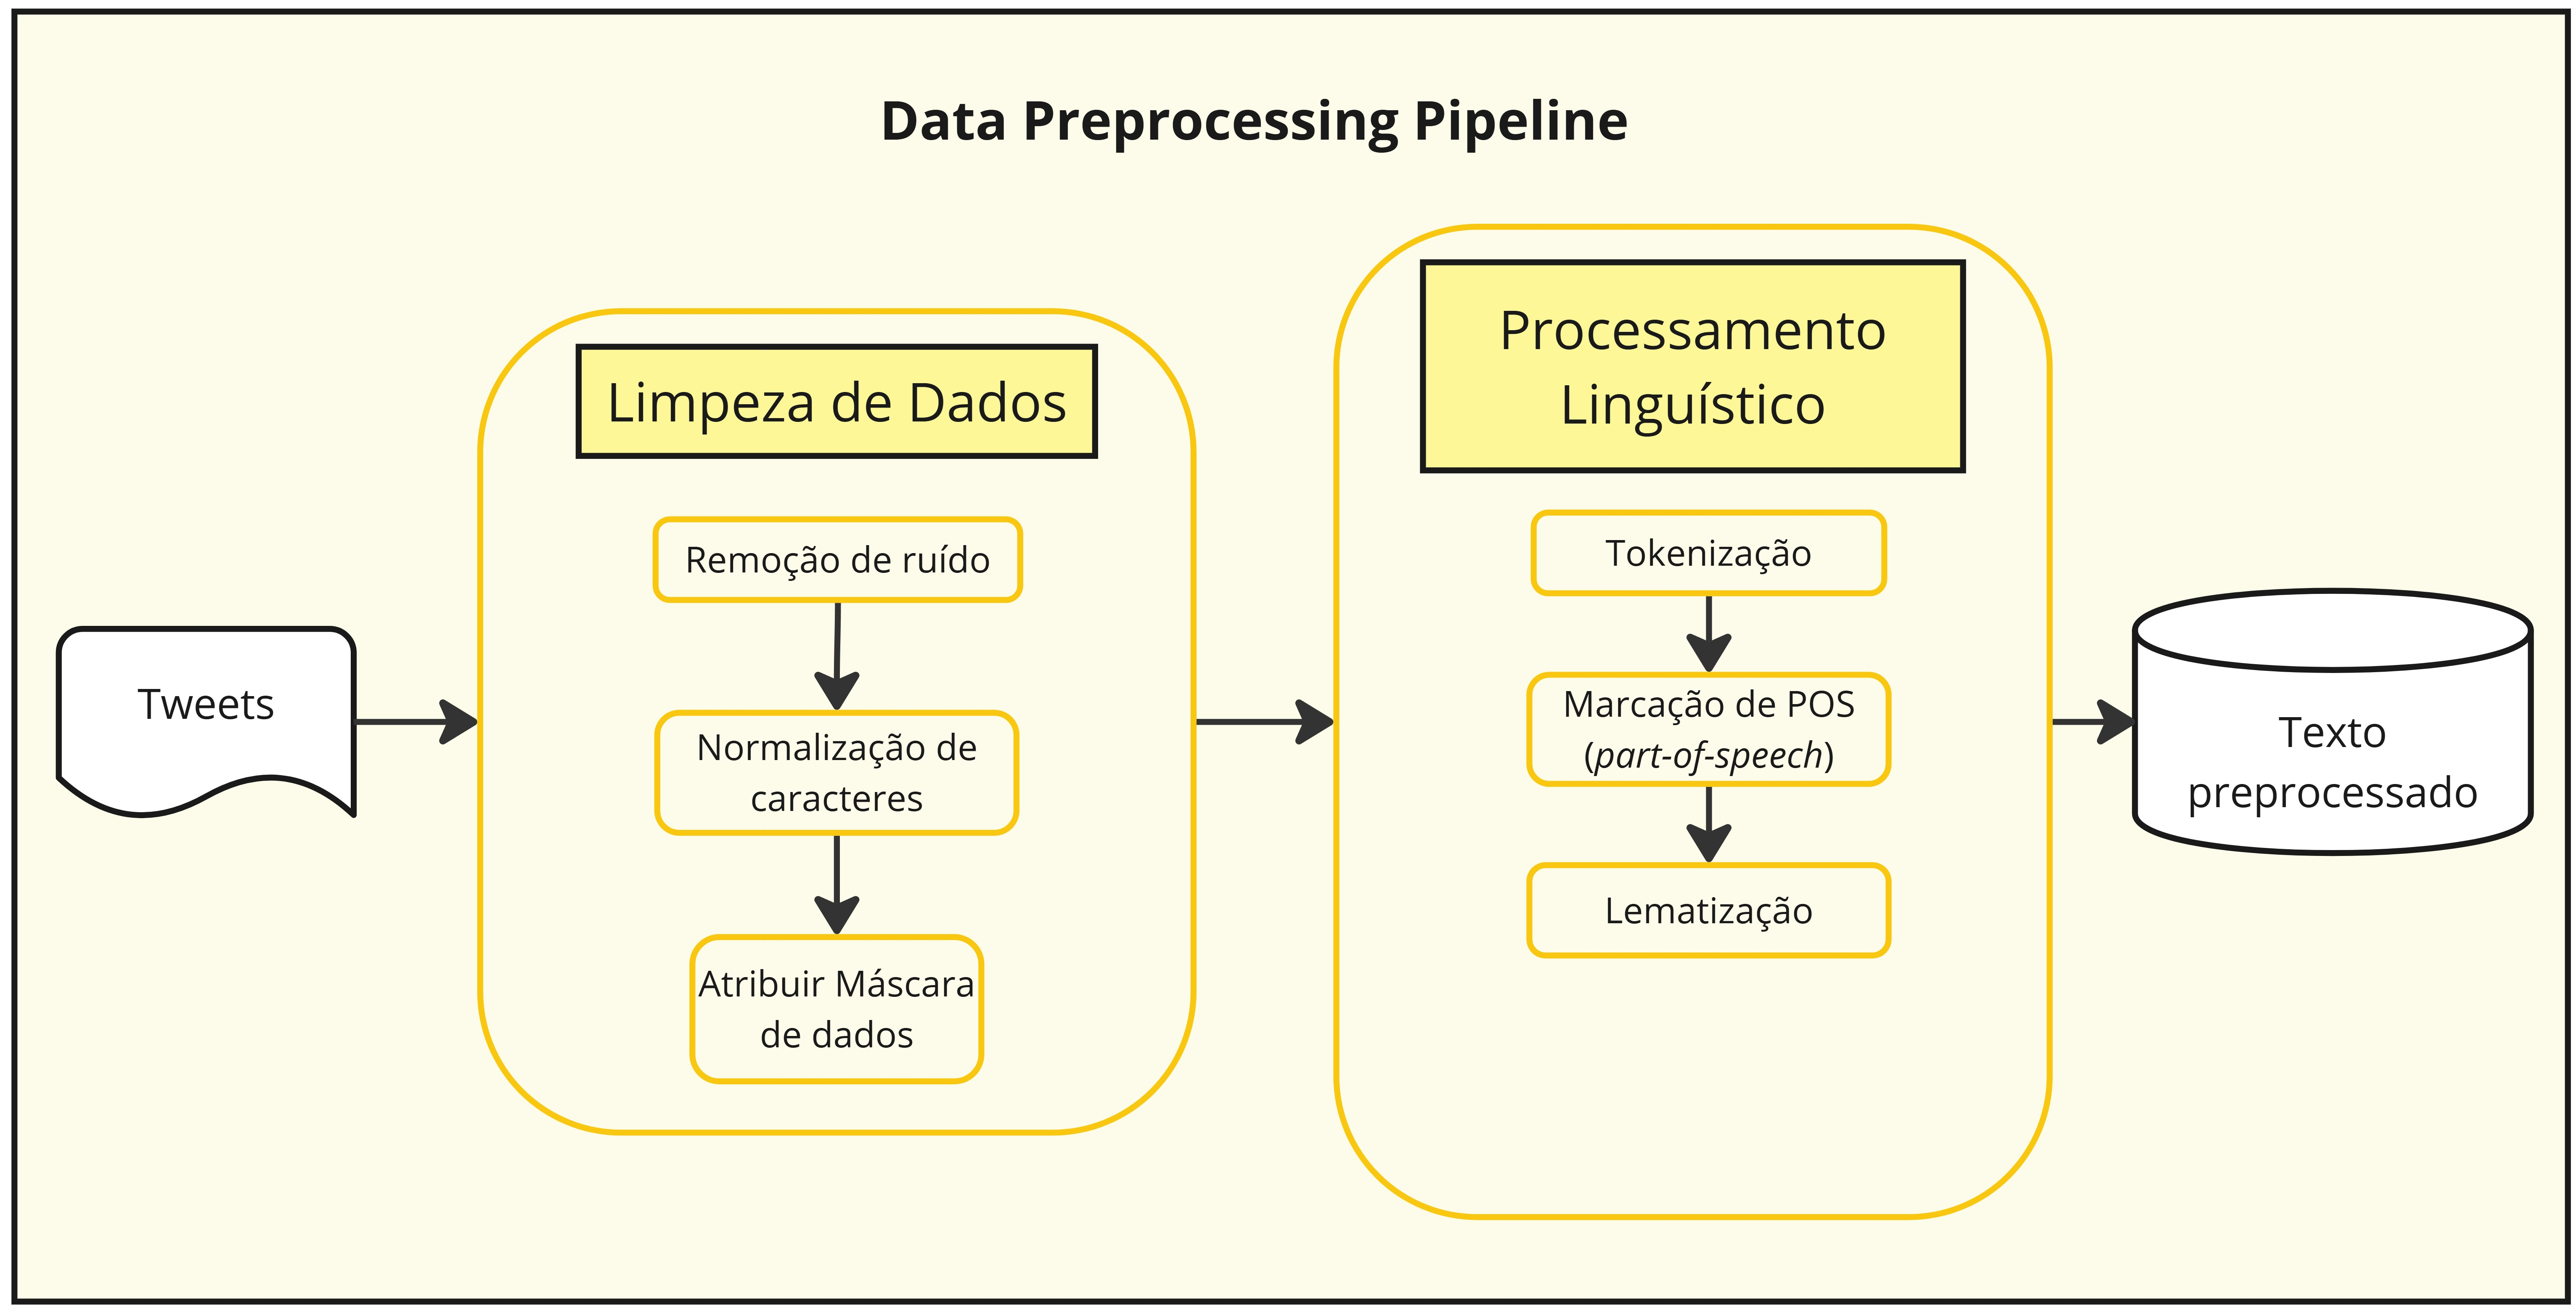
\includegraphics[scale=0.050]{imagens/figura_pipeline_preprocessamento_pt.jpg}
    \label{fig:pipeline_preprocessamento}
    \par\noindent
    \begin{minipage}{\textwidth}
        \centering
        \footnotesize % Adjust font size if needed
        \textit{Fonte: Elaboração própria}
    \end{minipage}
\end{figure}

A primeira tarefa do pré-processamento envolve a limpeza dos dados textuais. Essa atividade foi realizada por meio da Linguagem de Programação \textit{Python} em conjunto com os pacotes \textit{Spacy} e \textit{Textacy}, ambos referências dentro do ecossistema \textit{python} para aplicações que envolvam processamento linguístico. A limpeza de dados textuais é composta pelas das seguintes etapas:

\bigskip

1) Remoção de ruído: foram excluídos elementos não imprimíveis (\textit{non-printable}) e \textit{linebreakers}, tais como \textit{tags} HTML. Sequências de espaços foram substituídas por espaçamento simples. Foram ainda excluídas sequências isoladas de caracteres especiais - como \textit{\#?}, mas não \textit{\#covid-19}. 

\bigskip

2) Normalização de caracteres: textos foram convertidos para o formato \textit{unicode} (UTF-8), o que facilita sua manipulação. Acentos foram removidos e todas as letras foram formatadas enquanto minúsculas. Embora com tal estratégia envolva perda de informação (como ênfase por parte do usuário ao empregar letras maiúsculas), ganha-se com a redução de dimensionalidade dos dados. Aspas duplas e simples foram normalizadas para sua representação ASCII equivalente. Palavras que porventura tenham sido separadas por hífen durante a quebra de linhas foram reunidas.

\bigskip

3) Atribuir Máscara de Dados: Foi implementada uma máscara para elementos textuais que não denotam emoções, tais como URL's e endereços de e-mail. Emojis foram mantidos, pois um dos recursos linguísticos utilizados na etapa posterior consegue detectá-los e classificá-los quanto ao sentimento expressado.

\bigskip

Após a limpeza dos dados foi possível iniciar a tarefa de processamento linguístico. É importante ressaltar que as etapas dessa tarefa possuem um ordenamento necessário (i.e.: a lematização só pode ser realizada após a marcação de POS). O processamento linguístico possui as seguintes operações:

1) Tokenização: Refere-se à extração de \textit{tokens} dos documentos textuais. \textit{Tokens} são unidades semânticas - em contraposição às palavras (i.e.: \enquote{quarta-feira} possui duas palavras, mas juntas constituem uma unidade semântica). Os \textit{tokens} podem corresponder a uma palavra, sub-palavra ou conjunto de palavras desde que emitam um único significado. Estes elementos são os \textit{building blocks} dos modelos \textit{Large Language Models}, tal como o \textit{ChatGPT}. Sua extração envolve o emprego de um \textit{tokenizer}, que deve possuir conhecimento complexo da rede de regras que guiam uma determinada língua. Neste trabalho, foi utilizado o modelo de linguagem pre-treinado pt\_core\_news\_lg (541mb) disponível no pacote \textit{Spacy}. Seguindo a técnica empregada em \textcite{de_melo_comparing_2021} e \textcite{januario_sentiment_2022}, foram removidas as \textit{stop words} (i.e.: \enquote{para}, \enquote{já}, \enquote{que}, \enquote{no}) que não possuem significado próprio. Pontuações também foram removidas durante a tokenização.

\bigskip

2) Marcação de POS: \textit{Part-of-Speech tagging} é o processo de determinar a classe gramatical das palavras nos documentos textuais (i.e.: substantivo, verbo, artigos, adjetivos, etc.). Esse processo, por envolver o emprego de redes neurais, carregam algum grau de imprecisão devido ao caráter probabilístico desses modelos. Alguns estudos, tal como \textcite{de_melo_sentilexbr_2022}, após a realização da marcação de POS, optam por não trabalhar com substantivos por estes não carregarem conteúdo emotivo. Para este trabalho, optou-se por mantê-los.

\bigskip

3) Lematização: atividade que mapeia as palavras até sua forma não flexionada (i.e.: as palavras \enquote{ótimo}, \enquote{bom} e \enquote{melhor} são lexemas da palavra \enquote{bom}, da mesma forma que \enquote{tiver}, \enquote{tenho} e \enquote{tinha} são lexemas da palavra \enquote{tem}). A lematização requer a marcação de POS, uma vez que o lema de uma palavra está diretamente relacionado à sua classe gramatical. O uso da lematização ocasiona em perda de informação, como no caso entre \enquote{ótimo} e \enquote{bom}, que seriam ambos substituídos por apenas \enquote{bom}. Contudo, ganha-se em termos de redução da dimensionalidade dos dados.

\bigskip

Com a lematização, conclui-se o processamento linguístico e o \textit{dataset} pode ser atualizado conforme as informações obtidas (Ver Figura \ref{fig:dataset_preprocessado}). Preserva-se, assim, o texto original, juntamente com o texto \enquote{limpo}, os \textit{tokens} e os \textit{lemmas} na mesma base de dados. 

\begin{figure}[H]
    \captionsetup{position=above} % Coloca a legenda acima da imagem
    \caption{\textit{Dataset} da análise de sentimento}
    \centering
    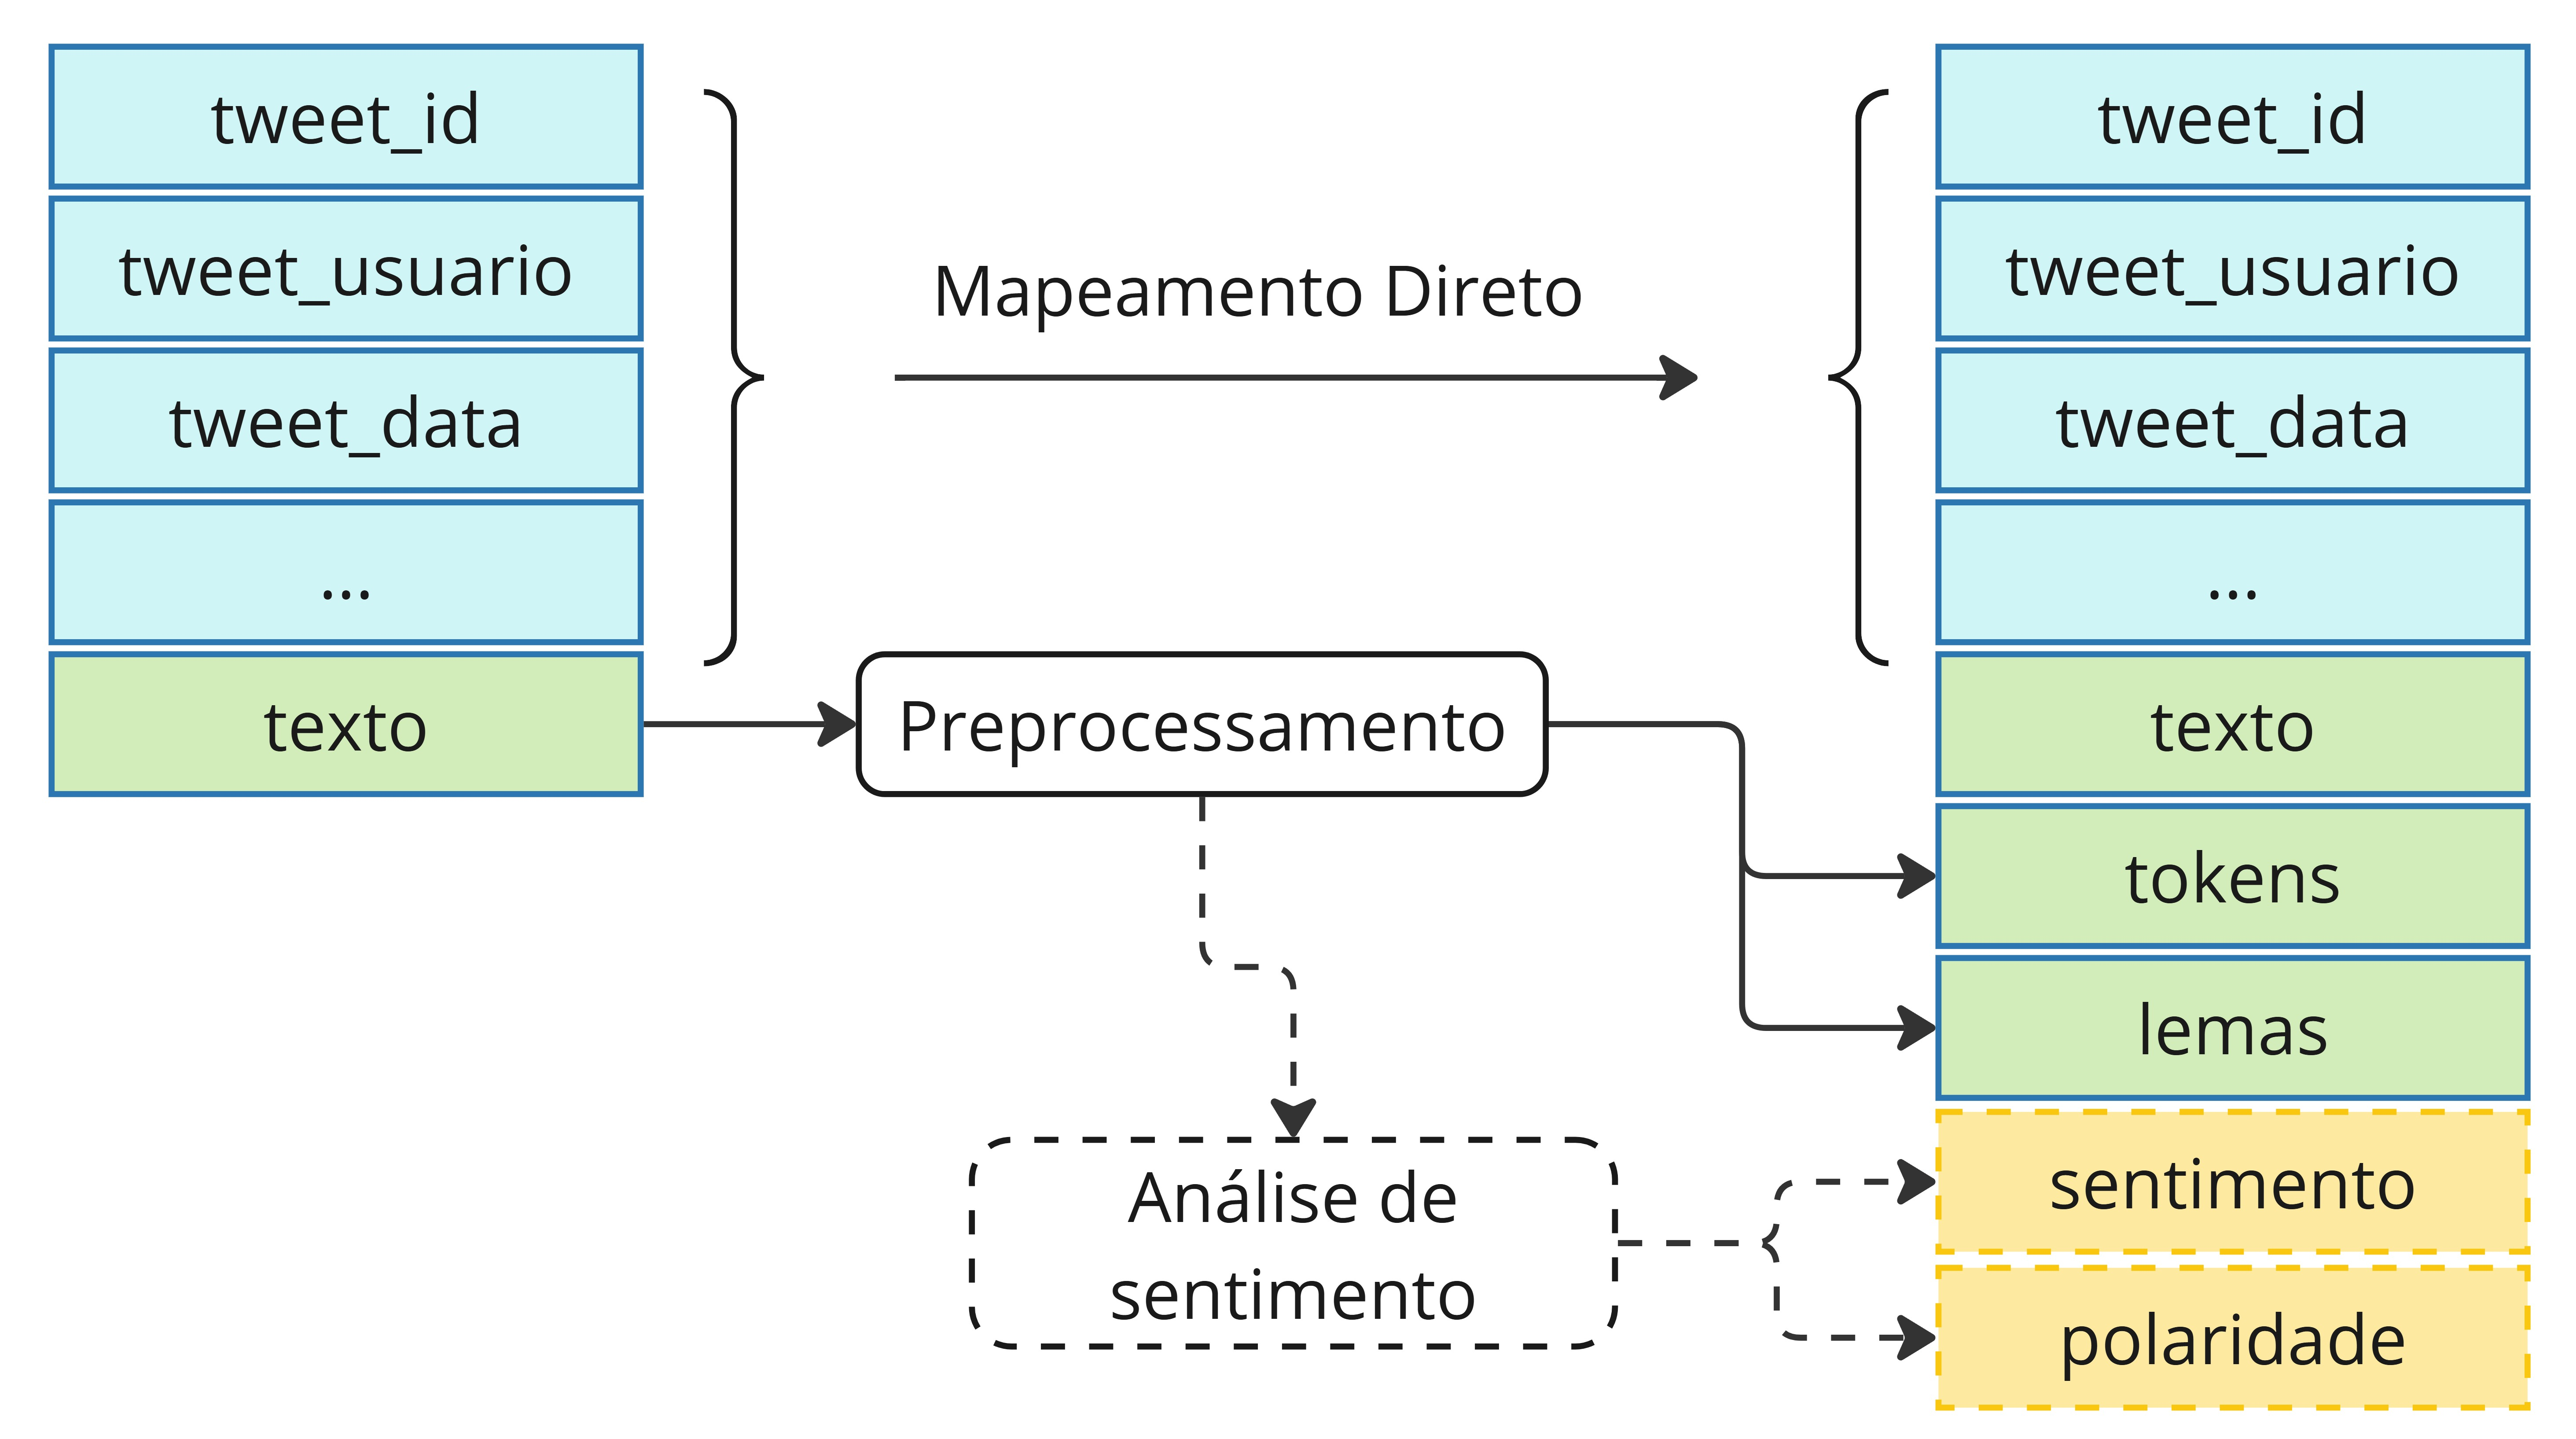
\includegraphics[scale=0.050]{imagens/figura_dataset_preprocessado.jpg}
    \label{fig:dataset_preprocessado}
        \par\noindent
    \begin{minipage}{\textwidth}
        \centering
        \footnotesize % Adjust font size if needed
        \textit{Fonte: Elaboração própria}
    \end{minipage}
\end{figure}

A próxima seção dedica-se à modelagem necessária para realização da análise de sentimento, que irá atribuir a cada \textit{tweet} um valor de sentimento correspondente, juntamente com a polaridade da publicação.



\bigskip

\textbf{Etapa 03: Modelagem}

A última etapa da análise de sentimento é a modelagem, que consiste no emprego de algoritmos para extração de sentimento dos \textit{tokens} e/ou \textit{lemmas} coletados durante a etapa de pré-processamento. Como optou-se pela abordagem léxica, é necessário o emprego dos léxicos enquanto recursos linguísticos adicionais sobre os quais os algoritmos se utilizam para atribuição de sentimento. 

Para essa seção, primeiro serão apresentados os léxicos empregados seguidos dos algoritmos para atribuição de sentimento e agregação dos dados. É importante ressaltar que a escolha dos léxicos seguiu os principais recursos utilizados em português do Brasil, conforme mapeados na \textit{survey} de \textcite{pereira_survey_2021}. Levou-se ainda em consideração a disponibilidade desses recursos de forma online e gratuita.

\subsection{Léxicos}

\bigskip
\subsubsection{OpLexicon}

É um léxico de propósito geral - em contraposição a um léxico de domínio específico que avalia a polaridade das palavras e \textit{tokens} segundo determinado contexto (i.e.: nas finanças) - elaborado por Souza e Vieira (2011). Possui 32.191 entradas, ou seja, termos classificados de acordo com a polaridade em que, em geral, são empregados, podendo ser positiva, negativa ou neutra. 

Alguns fatores justificam a utilização deste léxico, como o fato de ser um dos recursos linguísticos mais antigos e, consequentemente, mais utilizado pela literatura. Além disso, possui um número considerável de entradas em relação aos demais léxicos e foi citado como um dos léxicos mais importantes por \textcite{pereira_survey_2021}, que realizou uma \textit{survey} sobre os principais métodos e recursos linguísticos utilizados para análise de sentimento em português do brasil. 

Uma outra vantagem da aplicação deste léxico para o contexto de redes sociais é a presença de termos associados a \textit{emotions} e \textit{hastags}, formas comuns de expressão de emoções nesses ambientes. Entre os trabalhos mapeados na revisão de literatura que se utilizaram deste léxico estão \textcite{avanco_lexicon-based_2014} e \textcite{de_melo_sentilexbr_2022}.

\bigskip
\subsubsection{SentiLex}

É um léxico em língua portuguesa que adiciona especificação sintático-semântica aos termos nele contidos. Assim, o SentiLex incorpora as distintas conotações que uma mesma palavra pode assumir quando emprega junto à outra. Assim, por exemplo, o adjetivo \enquote{gordo} pode assumir conotação negativa enquanto modificador de natureza humana (i.e.: \enquote{indivíduo gordo}), mas polaridade positiva quando associado à palavra salário (i.e.: \enquote{salário gordo}).

O SentiLex possui dois léxicos associados, um que descreve os lemas e outro correspondente às formas flexionadas dos termos. Para este trabalho, optou-se por este último por ser mais completo, abarcando 18.098 termos que originam 36.286 formas flexionadas. O Sentilex foi desenvolvido por \textcite{carvalho_sentilex-pt_2015} e empregado nos trabalhos de \textcite{avanco_lexicon-based_2014} e \textcite{januario_sentiment_2022}. 

\bigskip
\subsubsection{Dicionário LM}

O dicionário LM, como é geralmente referenciado, inspirado no nome dos autores, \textcite{loughran_when_2010} é um léxico em inglês elaborado para análise de sentimento no contexto de economia e finanças. Por possuir um contexto específico de aplicação esse tipo de léxico é conhecido na literatura como \textit{domain-dependent}.

A justificativa de \textcite{loughran_when_2010}
para elaboração do dicionário LM é que muitas palavras identificadas com polaridade negativa em léxicos de propósito geral, não possuem essa conotação no domínio das finanças (i.e.: \textit{liability}). os autores mostram como 75\% das palavras identificação como negativa no \textit{Harvard Dictionary}, o principal léxico disponível em língua inglesa até então, não possuíam conotação negativa na área das finanças. 

Lançado em 2011 e, com última atualização em 2022, o dicionário LM tem sido extensivamente empregado pela literatura. Possui 86.531 entradas, apesar de apenas 2.692 estarem classificadas enquanto positivas ou negativas (as demais sendo neutras). O léxico traz ainda termos associados a outros espectros de polaridade como incerteza, litígio, que não serão utilizados neste trabalho a fim de facilitar a comparação com os demais léxicos utilizados. Utilizaram-se o léxico LM os trabalhos de \textcite{nyman_news_2021}, \textcite{shapiro_measuring_2020}, \textcite{shapiro_taking_2021}, \textcite{januario_sentiment_2022} e \textcite{picault_media_2022}. 

Como este recurso linguístico foi desenvolvido originalmente em inglês, a adaptação para o português pode ocorrer via tradução dos termos do dicionário - tal como \textcite{januario_sentiment_2022} ou dos documentos textuais - tal como \textcite{de_melo_sentilexbr_2022}. A tradução dos termos é a principal estratégia utilizada na literatura, devido a menor quantidade de termos a serem traduzidos, conferindo maior controle sobre o processo. 

Para o presente trabalho, optou-se pela tradução completa dos 86.531 termos contidos no dicionário LM através da API paga da empresa \textit{Open AI}, tendo sido utilizado o modelo \enquote{\textit{gpt-3.5-turbo}}. Devido ao fato de as palavras na língua portuguesa assumirem mais flexões do que na língua inglesa, construiu-se um \textit{prompt} que instruísse ao modelo incluir todas as variações de número e gênero das palavras, conforme a Figura \ref{fig:figura_chamada_api_openai}.


\begin{figure}[H]
    \captionsetup{position=above} % Coloca a legenda acima da imagem
    \caption{\textit{Snapshot} da função de tradução via API da \textit{OpenAI}}
    \centering
    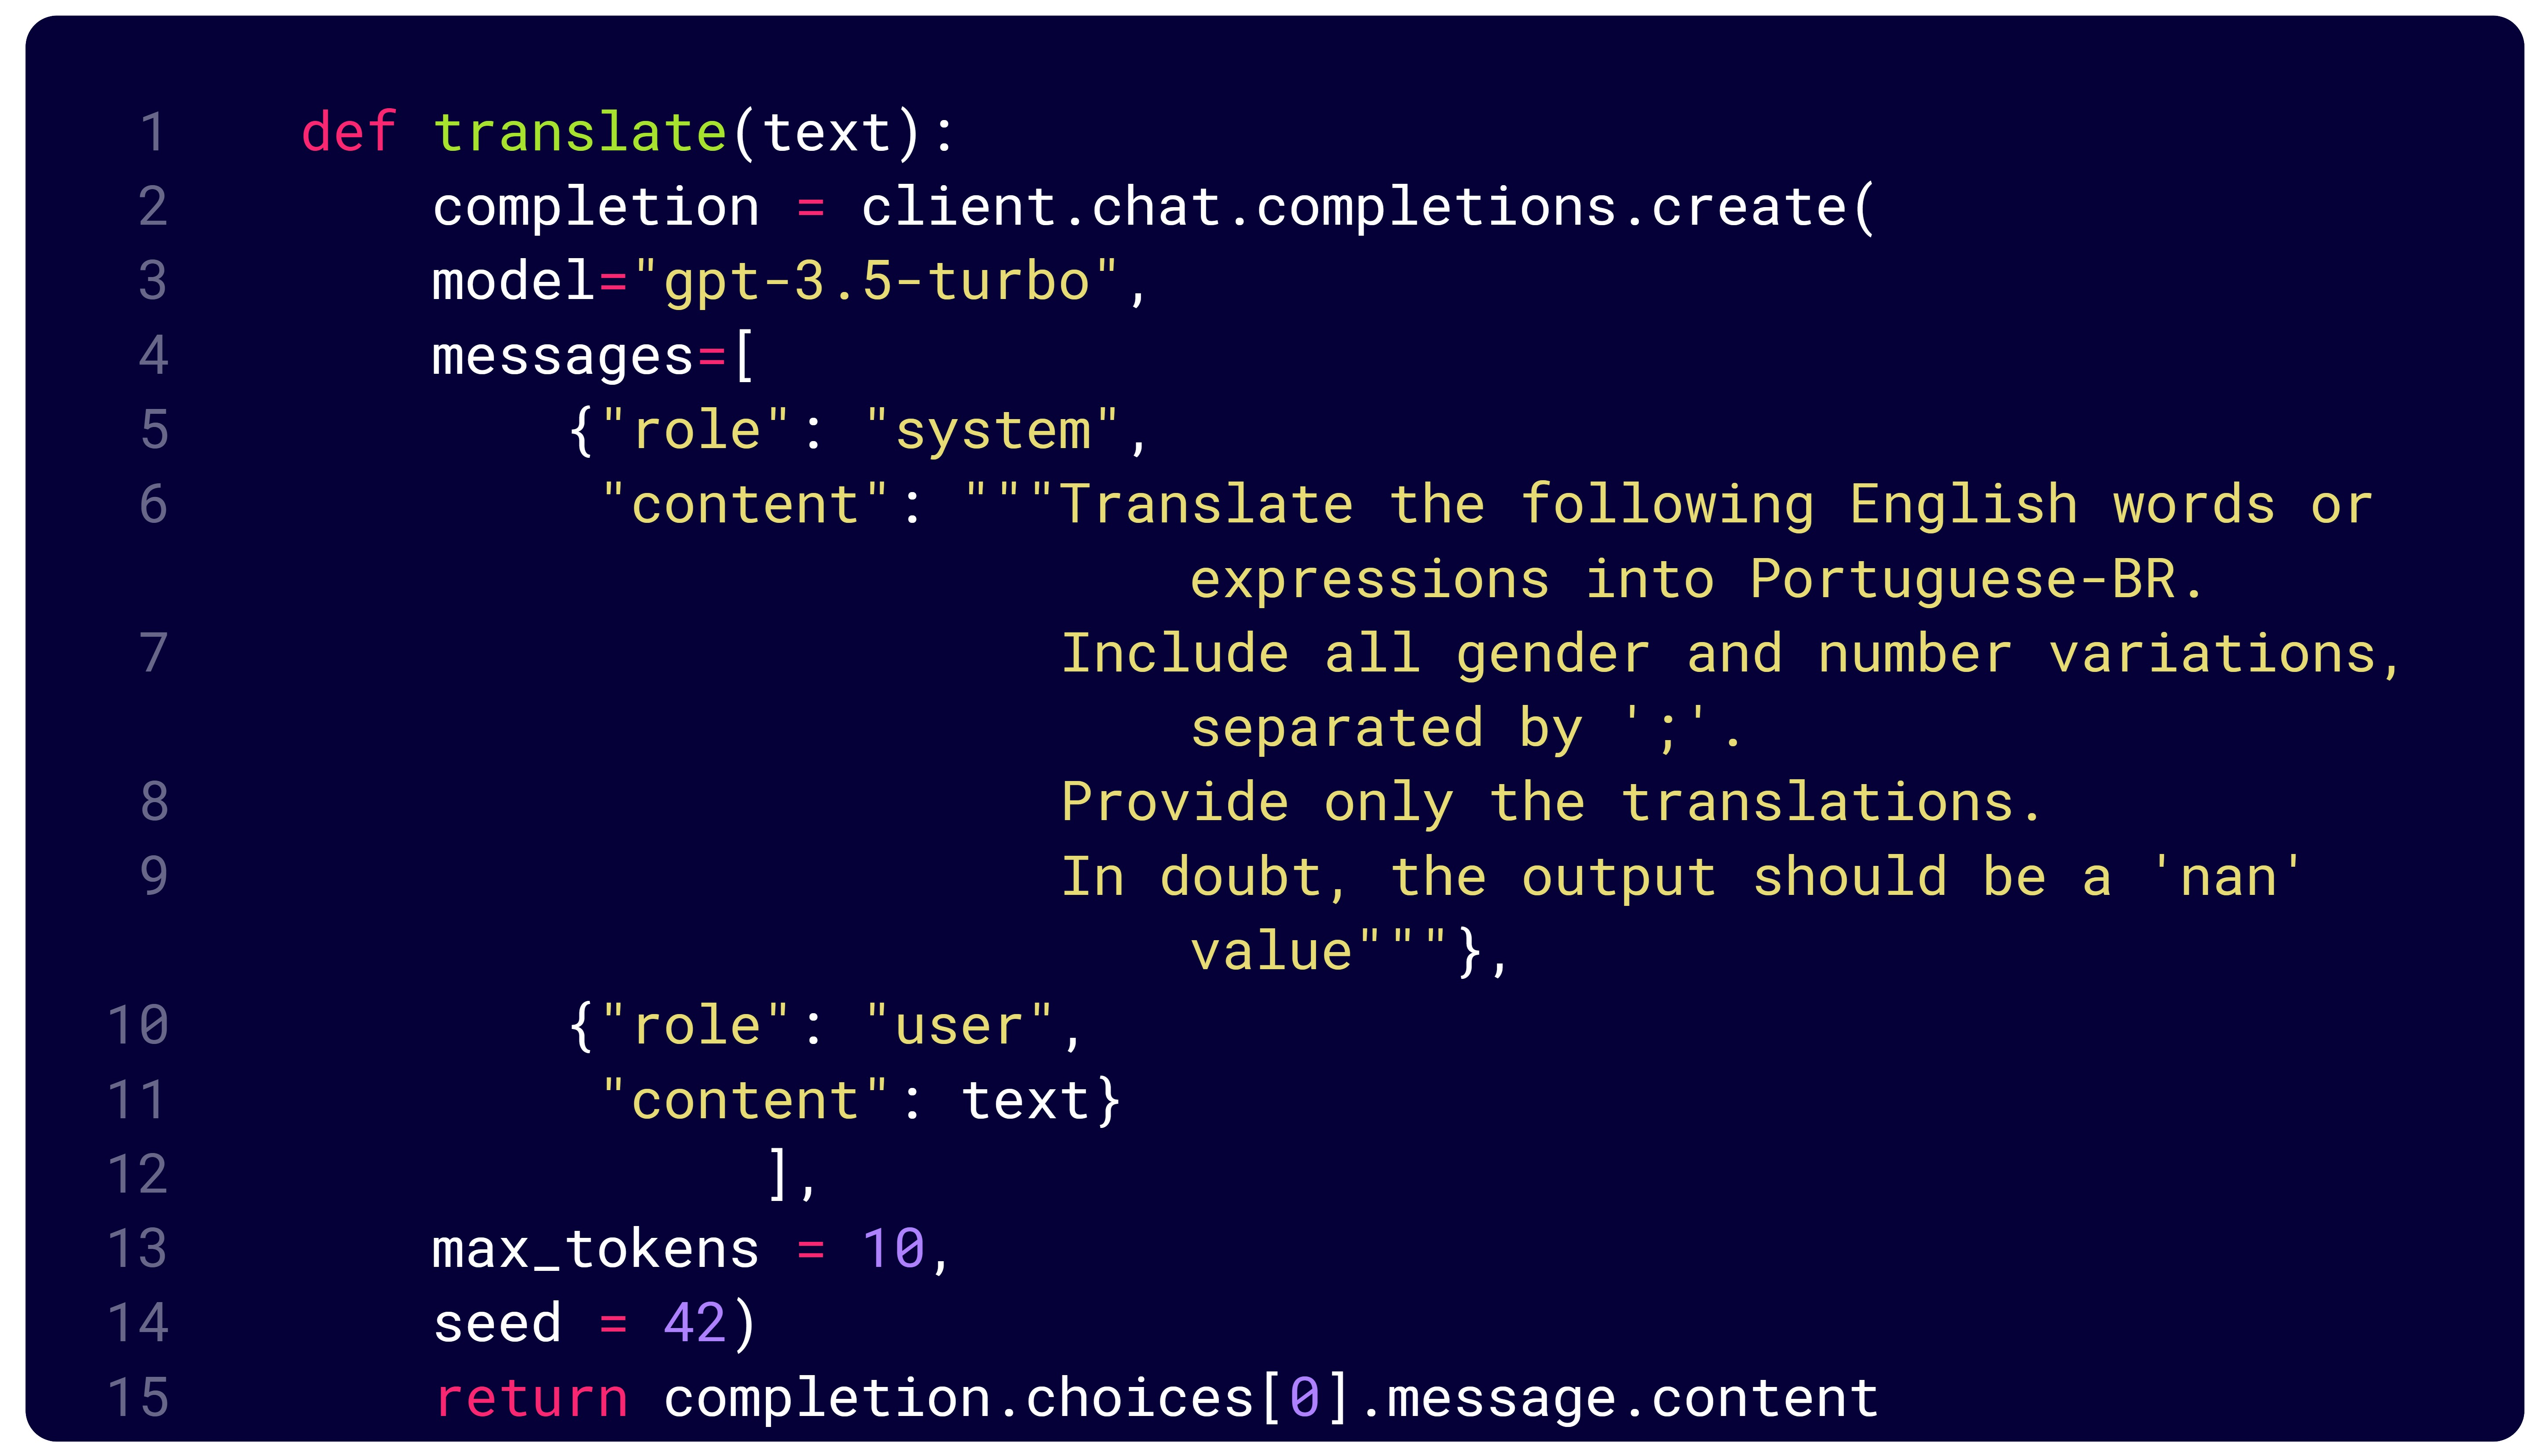
\includegraphics[scale=0.050]{imagens/figura_chamada_api_openai.jpg}
    \label{fig:figura_chamada_api_openai}
    \par\noindent
    \begin{minipage}{\textwidth}
        \centering
        \footnotesize % Adjust font size if needed
        \textit{Fonte: Elaboração própria}
    \end{minipage}
\end{figure}

Ao final do processo, algumas traduções aleatórias foram inspecionadas visualmente. Constatou-se a presença de alguns termos em português tanto com polaridade positiva quanto negativa, tendo sido esses termos excluídos do léxico traduzido, resultando em 493 termos com polaridade positiva e 3068 termos com polaridade negativa. 


\subsubsection{Vader}

Criado por \textcite{hutto_vader_2014}, o \textit{Valence Aware Dictionary and Sentiment Reasoner} (Vader), é um léxico em língua inglesa e, ao mesmo tempo, um atribuidor de \textit{scores} de sentimento para documentos textuais. À diferença dos demais léxicos, o Vader traz consigo um algoritmo de tipo determinístico (\textit{rule-based}), capaz de identificar contextos de negação (i.e.: \enquote{não gostei}) que invertem a polaridade das palavras e intensidade (i.e.: \enquote{muito bom}).

Os \textit{scores} atribuídos pelo Vader variam entre -1 (extremo negativo) e 1 (extremo positivo). Entre as vantagens do Vader para análise de sentimento neste trabalho está o fato de ter sido construído especificamente para captar sentimentos em redes sociais. Contudo, como esse recurso foi desenvolvido originalmente em inglês, foi necessário utilizar uma adaptação do léxico, sendo o recurso LEIA (Léxico para Inferência Adaptada), a principal ferramenta. Desenvolvida por \textcite{almeida_leia_2018}\footnote{https://github.com/rafjaa/LeIA. Último acesso em 23/08/2024.} e disponibilizada de maneira \textit{open source}, tem sido utilizada na literatura como em \textcite{marques_sentiment_2022} e \textcite{barreiro_implementacao_2023}. 

A Tabela \ref{tab:recursos_linguisticos} sintetiza as principais informações sobre os léxicos utilizados neste trabalho. 

\bigskip % Adiciona um espaço vertical (opcional)
\noindent
\begin{minipage}{\textwidth}
\centering
\captionof{table}{Recursos Linguísticos} % Legenda da tabela
\small % ou \footnotesize, \scriptsize, etc.
\begin{tabularx}{0.865\textwidth}{ % Ajuste o valor da largura total
>{\centering\arraybackslash}m{2.0cm}
>{\centering\arraybackslash}m{1.6cm}
>{\centering\arraybackslash}m{2.0cm}
>{\centering\arraybackslash}m{2.0cm}
>{\centering\arraybackslash}m{1.6cm}
>{\centering\arraybackslash}m{2.1cm}
}
\hline
\rowcolor{gray!20}
\textbf{Recurso Linguístico} & \textbf{Nº de Entradas} & \textbf{Finalidade} & \textbf{Autores} & \textbf{Formato} & \textbf{Última Atualização} \\ \hline
Op Lexicon & 32.191 & Propósito geral & \textcite{souza_sentiment_2012} & Léxico & 2012 \\ \hline
SentiLex & 36.286 & Propósito geral & \textcite{carvalho_sentilex-pt_2015} & Léxico & 2015 \\ \hline
LM & 85.531 & Propósito específico (finanças) & \textcite{loughran_when_2010} & Léxico & 2022 \\ \hline
Vader (LEIA) & 7.458 & Propósito geral & \textcite{hutto_vader_2014} & Léxico + Rule-Based & 2022 \\ \hline
\end{tabularx}
\label{tab:recursos_linguisticos} % Rótulo da tabela para referências
\vspace{0.2cm}
\par
    \begin{minipage}{\textwidth}
        \centering
        \footnotesize % Adjust font size if needed
        \textit{Fonte: Elaboração própria}
    \end{minipage}
\end{minipage}
\bigskip % Adiciona um espaço vertical (opcional)



\subsubsection{Algoritmos}



Os léxicos são recursos linguísticos no formato de um dicionário onde à cada palavra ou termo de um documento textual é atribuída uma polaridade. O algoritmo, por sua vez, é responsável por definir o conjunto de instruções que governam a forma como esses léxicos serão empregados na atribuição de polaridade (negativo/positivo) e \textit{score} (-1 até 1, em geral) para cada documento textual (i.e.: cada \textit{tweet}). A polaridade pode ser gradativa ao invés de binária, tal como o \textit{score} pode variar dentro de outro intervalo, mas esse formato especificado de expressar o sentimento é a maneira mais utilizada pela literatura.

É importante ressaltar que nesta seção serão abordadas duas aplicações necessárias dos algoritmos para análise de sentimento. A primeira refere-se aos algoritmos que pretendem atribuir sentimento a um documento textual. A segundo refere-se à fórmula utilizada para agregação do sentimento num intervalo de tempo. 

A forma geralmente empregada pela literatura para atribuição e um valor que represente o sentimento de um documento textual envolve a ponderação entre o número de palavras positivas e negativas presentes em cada documento. Em geral, a subtração do número de palavras positivas pelo número de palavras negativas sobre o número total de palavras fornece um indicador que informa tanto sobre a valência (negativo/positivo) quanto à intensidade do sentimento. 

O Algoritmo \ref{algo:algoritmo_sentimento} detalha a construção do indicador de sentimento \(S_d\) para cada \textit{tweet}, utilizando um léxico qualquer enquanto provedor de polaridade dos \textit{tokens}. 

\bigskip
\textbf{Insumo:}
\begin{itemize}
    \item \textbf{Vocabulário do Léxico} \( V = \{w_1, w_2, \ldots, w_m\} \);
    \item \textbf{Pares} \( L = \{\langle w_1, p\rangle, \langle w_2, p\rangle, \ldots, \langle w_m, p\rangle\} \), onde \( w_i \in V \) e \( p \in \{\text{positivo}, \text{negativo}\} \);
\end{itemize}

\textbf{Produto:}
\begin{itemize}
    \item \textbf{Sentimento do documento} \( S_d \): um valor numérico representativo do sentimento do documento \(d\).
\end{itemize}

\begin{algorithm}
\caption{Cálculo de Sentimento do Documento} % Título do algoritmo
\label{algo:algoritmo_sentimento}
\begin{algorithmic}[1]
    \State \textbf{let} \( L^+ \) \textbf{be} o conjunto de tokens positivos \( L^+ = \{w_i \mid p = \text{positivo}\} \);
    \State \textbf{let} \( L^- \) \textbf{be} o conjunto de tokens negativos \( L^- = \{w_i \mid p = \text{negativo}\} \);
    \State \textbf{let} \( S_d = 0 \);
    \State \textbf{let} \( W_d = \{w_1, w_2, \ldots, w_n\} \) \textbf{be} o conjunto de tokens do documento \(d\);
    \For{\textbf{each} \( w_i \in W_d \)}
        \If{\( w_i \in L^+ \)}
            \State \( S_d = S_d + 1 \);
        \ElsIf{\( w_i \in L^- \)}
            \State \( S_d = S_d - 1 \);
        \Else
            \State \textbf{continue};
        \EndIf
    \EndFor
    \State \( S_d =  \frac{S_d}{\text{lenght}(W_d)} \)
    \State \Return \(S_d\);
\end{algorithmic}
\end{algorithm}
\vspace{-0.8cm}
\par\noindent
    \begin{minipage}{\textwidth}
        \centering
        \footnotesize % Adjust font size if needed
        \textit{Fonte: Elaboração própria}
    \end{minipage}
\bigskip

A fórmula do Algoritmo \ref{algo:algoritmo_sentimento} segue aquela adotada por \textcite{shapiro_taking_2021} e \textcite{picault_media_2022}, onde para cada \textit{token} positivo em um documento textual, adiciona-se 1 e para cada \textit{token} negativo, subtrai-se 1. Ao final, a variável de sentimento é dividida pelo número de \textit{tokens} no documento textual, garantindo que o indicador de sentimento por documento assuma valores no intervalo \( [-1, 1]\).

Esse formato de cálculo, contudo, tem uma limitação: todos os \textit{tokens} possuem o mesmo peso. Como os léxicos apontam apenas a polaridade dos termos, tem-se que \enquote{ruim} e \enquote{terror} impactam igualmente o indicador. Alguns trabalhos recentes têm proposto algoritmos e outros recursos linguísticos a fim de atribuir diferentes \textit{scores} entre as palavras, permitindo estabelecer uma diferenciação quanto à intensidade das emoções. São exemplos de trabalhos nesse sentido \textcite{mello_combining_2022} e \textcite{marques_sentiment_2022}. Essa opção, contudo, não faz parte do escopo deste trabalho.

A Tabela \ref{tab: termos_pos_neg_lexicos}, juntamente com exemplos apresentados em seguida, evidenciam a operação do algoritmo no processo de extrair sentimento dos \textit{tweets} de acordo com os léxicos empregados. É importante ressaltar, contudo, que a aplicação do VADER não se utiliza do algoritmo, uma vez que a ferramenta possui um conjunto de instruções próprio para atribuição de sentimento. 


\begin{table}[h]
\centering
\caption{Identificação de termos positivos e negativos pelos léxicos (exemplos)}
\label{tab: termos_pos_neg_lexicos}
\begin{adjustbox}{max width=\textwidth}
    \begin{tabular}{|l|l|}
    \hline
    \rowcolor[HTML]{EFEFEF} 
    \textbf{Formato do texto} & \textbf{Significado} \\ \hline
    \textcolor{blue}{em azul} & Palavras positivas em pelo menos um dicionário (e quais dicionários)\\ \hline
    \textcolor{red}{em vermelho} & Palavras negativas em pelo menos um dicionário (e quais dicionários)\\ \hline
    \end{tabular}
\end{adjustbox}
\vspace{0.2cm}
\par\noindent
    \begin{minipage}{\textwidth}
        \centering
        \footnotesize % Adjust font size if needed
        \textit{Fonte: Elaboração própria}
    \end{minipage}
\end{table}

\bigskip


\textit{Tweet 01 - Data: 2017-05-18 08:36:20} \\
\enquote{O Banco Central (...) atuará para manter a \textcolor{blue}{$\underset{\text{(Op)}}{\text{plena}}$} funcionalidade dos mercados} - pode atuar no dólar e comprar títulos! \textcolor{blue}{$\underset{\text{(Op, SL, LM)}}{\text{Excelente}}$} BC!! \\
\textit{\small Índice de Sentimento: Op = 0.07; SentiLex = 0.04; LM = 0.04; VADER = 0.53}

\bigskip
\bigskip

\textit{Tweet 02 - Data: 2021-02-08 20:09:48	} \\
A aprovação do projeto de lei sobre \textcolor{blue}{$\underset{\text{(SL)}}{\text{autonomia}}$} do Banco Central, \textcolor{blue}{$\underset{\text{(Op)}}{\text{previsto}}$} para ser votado na Câmara nesta semana, dará uma mensagem \textcolor{blue}{$\underset{\text{(LM*)}}{\text{muito}}$} \textcolor{blue}{$\underset{\text{(Op, SL, LM)}}{\text{positiva}}$} para o mercado	\\
\textit{\small Índice de Sentimento: Op = 0.14; SentiLex = 0.04; LM = 0.07; VADER = 0.05} \\
{\textit{\small *Para o dicionário LM, o termo \enquote{muito} só apresenta polaridade positiva quando em conjunto com o termo \enquote{positiva} ou \enquote{positivo}.}}

\bigskip
\bigskip

\textit{Tweet 03 - Data: 2020-02-10 13:55:43} \\
Vamos \textcolor{red}{$\underset{\text{(LM)}}{\text{combinar}}$}, o juro \textcolor{blue}{$\underset{\text{(Op, SL)}}{\text{real}}$} não baixou. Baixou o nominal por \textcolor{red}{$\underset{\text{(SL, LM)}}{\text{falta}}$} de demanda e atividade \textcolor{blue}{$\underset{\text{(Op, SL)}}{\text{produtiva}}$}, \textcolor{red}{$\underset{\text{(SL, LM)}}{\text{desemprego}}$} e salários \textcolor{red}{$\underset{\text{(Op, SL)}}{\text{congelados}}$}. Na Antártica também não há inflação, e nenhuma atividade \textcolor{blue}{$\underset{\text{(SL)}}{\text{econômica}}$}. \\
\textit{\small Índice de Sentimento: Op = 0.05; SentiLex = 0.00; LM = -0.09; VADER = -0.61}

\bigskip
\bigskip

Após a atribuição de um valor de sentimento para cada \textit{tweet} pelo Algoritmo \ref{algo:algoritmo_sentimento}, é necessário promover a agregação do sentimento para um determinado intervalo temporal. 

Tal como ocorre com os dados textuais de noticiários, as redes sociais apresentam muito ruído de informação, com agregações de alta frequência como dias ou semanas, apresentando resultados com alta volatilidade. Além disso, a maior parte dos dados econômicos com os quais procura-se confrontar os índices de sentimento, possuem periodicidade mensal ou trimestral, tendo sido esses intervalos os mais empregados pela literatura. Para este trabalho, optou-se por prosseguir com a agregação mensal.

Existem duas principais fórmulas, bem como variações decorrentes de cada uma delas, encontradas na literatura para agregar o sentimento de documentos textuais publicados em um intervalo \(t\):

% Using equation environment for numbered equations
\begin{equation}
\label{eq:sentiment_picault}
\text{Sentiment}_t = \frac{\sum \text{Sentiment}_i}{N_t}
\end{equation}

\begin{equation}
\label{eq:sentiment_carosia}
\text{Sentiment}_t = \frac{N(\text{pos}) - N(\text{neg})}{N(\text{pos}) + N(\text{neg})}
\end{equation}

A equação \ref{eq:sentiment_picault} apresenta a primeira dessas fórmulas, que é apenas o cálculo da média aritmética do sentimento em todos os \textit{tweets}. Soma-se o valor do sentimento de cada \textit{tweet} \(i\) e divide-se pelo número total de \textit{tweets} no intervalor \(t\). Essa fórmula foi utilizada nos trabalhos de \textcite{de_melo_comparing_2021} e \textcite{picault_media_2022}, possuindo ainda semelhança com a utilizada em \textcite{nyman_news_2021}.

A equação \ref{eq:sentiment_carosia} é a divisão entre a diferença do número de \textit{tweets} positivos e negativos sobre sua soma, tal como empregado em \textcite{carosia_analyzing_2020}. Antes de realizar essa operação, contudo, é necessário identificar os \textit{tweets} positivos e negativos. Para isso, geralmente utiliza-se o valor do sentimento atribuído a cada \textit{tweet}, sendo negativo se menor do que zero, positivo se maior do que zero e neutro se igual à zero, como em \textcite{mello_combining_2022} e \textcite{januario_sentiment_2022}.  

\clearpage
\section{Séries Temporais}
\label{metodologia_series_temporais}


O principal uso de um índice de sentimento tem sido seu emprego em modelagens de séries temporais a fim de avaliar seu poder preditivo e/ou explanatório sobre outras variáveis de interesse. 

No domínio da economia e das finanças, o modelo VAR (\textit{Vector Autoregression)} destaca-se como principal forma de modelar um índice de sentimento com variáveis econômicas, tais como juros, PIB, inflação, dentre outras. 


\subsection{O modelo VAR}


É conveniente a representação desse modelo através de um VAR de ordem 1 bivariado, conforme \textcite{enders_applied_2015}. Assim, seja o seguinte sistema de equações de um VAR(1):

\begin{align*}
z_t  &= b_{10} - b_{12} y_t + \gamma_{11} z_{t-1} + \gamma_{12} y_{t-1} + \varepsilon_{zt}, ~~~~\varepsilon_{zt} \sim \mathcal{RB}(0, \sigma^2_z) 
\\
y_t &= b_{20} - b_{21} z_t + \gamma_{21} z_{t-1} + \gamma_{22} y_{t-1} + \varepsilon_{yt}, ~~~~\varepsilon_{yt} \sim \mathcal{RB}(0, \sigma^2_y)
\end{align*}

onde os vetores de perturbações aleatórias \(\varepsilon_{zt}\) e \(\varepsilon_{yt}\) seguem um processo ruído branco com média zero e variância finita. Por construção, nesse sistema, \( z_t \) é afetada por seus valores passados e pelos valores contemporâneos e passados de  \( y_t \). Do efeito contemporâneo (efeito \textit{feedback}) que uma variável exerce sobre a outra emerge o viés de equação simultânea: com regressores e termos de erro sendo correlacionados (i.e.: \( y_t \) e  \(\varepsilon_{zt}\)), estimações dos parâmetros por MQO são viesadas e inconsistentes.

A solução passa por estimar uma forma reduzida do modelo. Sejam as equações anteriores apresentadas em sua forma matricial:
\begin{equation}
\underbrace{\begin{bmatrix} 1 & b_{12} \\ b_{21} & 1 \end{bmatrix}}_{\equiv B}
\underbrace{\begin{bmatrix} z_t \\ y_t \end{bmatrix}}_{\equiv X_t}
=
\underbrace{\begin{bmatrix} b_{10} \\ b_{20} \end{bmatrix}}_{\equiv \Gamma_0}
+
\underbrace{\begin{bmatrix} \gamma_{11} & \gamma_{12} \\ \gamma_{21} & \gamma_{22} \end{bmatrix}}_{\equiv \Gamma_1}
\underbrace{\begin{bmatrix} z_{t-1} \\ y_{t-1} \end{bmatrix}}_{\equiv X_{t-1}}
+
\underbrace{\begin{bmatrix} \varepsilon_{zt} \\ \varepsilon_{yt} \end{bmatrix}}_{\equiv \varepsilon_t}
\end{equation}

Em notação compacta, a seguinte equação descreve a forma estrutural do VAR:

\begin{equation}
BX_t = \Gamma_0 + \Gamma_1X_{t-1} + \varepsilon_t
\end{equation}

onde \(X_t\) representa o vetor de variáveis endógenas. Multiplicando-se ambos os termos da equação por \( B^{-1}\), tem-se a forma reduzida do VAR:

\begin{equation}
X_t = A_0 + A_1X_{t-1} + e_t, 
\end{equation}

\begin{equation}
\left\{ 
\begin{array}{l}
A_0 \equiv B^{-1}\Gamma_0, \\
A_1 \equiv B^{-1}\Gamma_1, \\
e_t \equiv B^{-1}\varepsilon_t
\end{array} 
\right.
\end{equation}

onde os parâmetros do modelo podem ser estimados uma vez atendida a condição de estabilidade, ou seja, os autovalores da polinomial \((I - A_1L)\) se localizarem fora do círculo unitário.

A forma reduzida do VAR permite a estimação direta dos parâmetros de cada equação por MQO, produzindo estimadores assintoticamente eficientes e consistentes \textcite{enders_applied_2015}. Isso pois, a manipulação algébrica, permite eliminar o efeito \textit{feedback} da forma estrutural. Vale ressaltar, contudo, que tal resultado só se sustenta quando se assume que os erros são serialmente não correlacionados. Assim:

\begin{equation}
\varepsilon_{zt} \perp \varepsilon_{yt} \implies \text{Cov}(\varepsilon_{zt}, \varepsilon_{yt}) = 0
\end{equation}

Apesar de ser possível a estimação da forma reduzida, a questão central da utilização do VAR para modelagem de variáveis econômicas reside na possibilidade de, através dos parâmetros da forma reduzida, recuperar os parâmetros estruturais. Isso pois, apenas no modelo em sua forma estrutural, seria possível isolar os efeitos dos choques e identificar relações contemporâneas entre as variáveis.

A recuperação dos parâmetros é possível devido à equivalência algébrica entre a forma reduzida e a forma estrutural. Contudo, a forma estrutural é sobreparametrizada com relação à forma reduzida, sendo necessária a imposição de restrições adicionais ao modelo para identificação exata entre as duas formas.

Uma vez estimados os resíduos na forma reduzida, as restrições adicionais devem ser incorporadas na matriz \(B\) de forma a preservar a independência dos resíduos no sistema estrutural e identificar a relação:

\begin{equation}
e_t \equiv B^{-1}\varepsilon_t
\end{equation}


Convém avaliar a matriz de covariância dos resíduos para identificar o número de restrições necessárias. 

\begin{equation}\Sigma = \begin{bmatrix}
\sigma_{11}^2 & \sigma_{12} & \cdots & \sigma_{1n} \\
\sigma_{21} & \sigma_{22}^2 & \cdots & \sigma_{2n} \\
\vdots & \vdots & \ddots & \vdots \\
\sigma_{n1} & \sigma_{n2} & \cdots & \sigma_{nn}^2 
\end{bmatrix}\end{equation}

onde cada elemento  \(\sigma_{ij}\) é estimado por:

\begin{equation}
\sigma_{ij} = \frac{1}{T} \sum_{t=1}^{T} e_{it}e_{jt}
\end{equation}

Por ser simétrica, a matriz \(\Sigma\) apresenta \( n(n+1)/2\) elementos distintos e passíveis de serem conhecidos pela estimação do VAR na forma reduzida. Na forma estrutural, desconhecem-se \((n^2-n)\) elementos da matriz \(B\), uma vez que os elementos de sua diagonal são unitários, além dos \(n\) valores relativos à variância dos vetores \(\varepsilon_t\). Assim, é necessária a imposição de \((n^2-n + n) - n(n+1)/2 = n(n-1)/2\) restrições ao modelo estrutural. 

Existem duas estratégias comumente empregas para identificação do VAR estrutural: i) a Decomposição de Cholesky; ii) o estabelecimento de restrições de acordo com a teoria econômica.

A Decomposição de Cholesky se utiliza de uma matriz triangular superior para identificação exata do modelo estrutural. Como nesse tipo de matriz, todos os elementos da diagonal superior são zeros, resulta-se que, para um sistema de \(n\) variáveis endógenas, são estabelecidas \((n^2-n)/2\) restrições. Exatamente o número necessário para, através da estimação do VAR reduzido, recuperar os parâmetros do VAR estrutural. 

Seja a relação entre resíduos estimados e erros estruturais do exemplo em questão:

\begin{equation}\begin{bmatrix}e_{1t} \\e_{2t}
\end{bmatrix}\equiv B^{-1}\varepsilon_t =\begin{bmatrix}
\frac{\varepsilon_{zt} - b_{12} \varepsilon_{yt}}{1 - b_{12}b_{21}} \\[5pt]\frac{\varepsilon_{yt} - b_{21} \varepsilon_{zt}}{1 - b_{12}b_{21}}\end{bmatrix}
\end{equation}

Da decomposição de Cholesky, em que \(B = \begin{bmatrix} 1 & 0 \\ b_{21} & 1 \end{bmatrix}\), resulta que: 


\begin{equation}\begin{aligned}
    e_{1t} &= \varepsilon_{zt} \\
    e_{2t} &= \varepsilon_{yt} - b_{21}\varepsilon_{zt}
\end{aligned}\end{equation}

onde apenas os choques \(\varepsilon_{zt}\) de \(z_t\) a afetam contemporaneamente, enquanto \(y_t\) é influenciada tanto por \(\varepsilon_{zt}\) quanto por \(\varepsilon_{yt}\). Daí \(z_t\) ser dita \textit{"causally prior"} em relação à \(y_t\). Dessa assimetria que emerge entre as variáveis endógenas é necessário algum fundamento teórico que justifique seu ordenamento no sistema de equações. 

A outra estratégia para identificação do VAR reside no estabelecimento de restrições advindas da teoria econômica. Advogam em favor dessa estratégia autores como \textcite{sims_are_1986}, \textcite{bernanke_alternative_1986} e \textcite{blanchard_dynamic_1988}. Convencionou-se denominar essa estratégia como \textit{Structural VAR} (ou SVAR) à diferença de apenas VAR, uma vez que, em geral, a estimação dos parâmetros estruturais nessa última denominação se dá por Decomposição de Cholesky.

Contra a Decomposição de Cholesky, esses autores invocam a forte suposição relativa à decomposição dos erros resultante, qual seja, a de que o verdadeiro processo gerador de dados obedece à estrutura definida por uma matriz triangular superior. Outra crítica comum é a inviabilidade de se testar todos os ordenamentos possíveis. 

Desde que satisfeito o número mínimo de restrições necessárias para compatibilizar o VAR reduzido com o VAR estrutural, a estratégia de identificação do tipo SVAR pode, ainda, impor novas restrições à matriz \(B\) em acordo com a teoria subjacente, resultando em um modelo sobre-identificado. Essa opção, contudo, deve ser avaliada com cuidado, pois caso as restrições imponham muitos valores nulos aos coeficientes \(b_{ij}\), a matriz \(B\) pode tornar-se não invertível. 

Assim, o SVAR impõe um modelo econômico teórico à estrutura dos dados em séries temporais. O aspecto central desse modelo é a influência contemporânea dos termos de erro estruturais, também referidas como inovações estruturais, nas variáveis endógenas do sistema. 

Uma vez definida a estratégia de identificação e estimados os parâmetros do modelo estrutural, o VAR per se tem pouca utilidade prática. Grande parte do interesse de pesquisa desse modelo reside na construção das Funções de Resposta-Impulso (FRI) e nas Decomposições de Variância, derivadas do VAR. Ambas permitem a identificação de regularidades empíricas que sustentam modelos teóricos em economia \parencite{jorda_estimation_2005}. 


\subsection{Funções de Resposta Impulso (FRI)}


Interesse particular neste trabalho é depositado na estimação das FRI, que permitem rastrear o impacto de choques estruturais nas variáveis endógenas do modelo. Seguindo a notação empregada por \textcite{enders_applied_2015} e repetindo a notação exposta acima por conveniência, seja o modelo VAR em sua forma reduzida e compacta dada por: 

\begin{equation}
X_t = A_0 + A_1X_{t-1} + e_t, 
\end{equation}

ou em notação matricial: 

\begin{equation}\begin{aligned} \begin{bmatrix}
        z_t \\ y_t \end{bmatrix} &=\begin{bmatrix}
        a_{10} \\ a_{20}\end{bmatrix} +
    \begin{bmatrix}a_{11} & a_{12} \\a_{21} & a_{22}
    \end{bmatrix}\begin{bmatrix} z_{t-1} \\ y_{t-1}
    \end{bmatrix}  +\begin{bmatrix} e_{1t} \\ e_{2t}
    \end{bmatrix}\end{aligned}\end{equation}

Satisfeita a condição de estabilidade, ou seja,  os autovalores da polinomial \((I - A_1L)\) estando fora do círculo unitário no plano complexo, um modelo \(VAR(P)\) possui representação \(VMA(\infty)\) - tal como um \(AR(P)\) possui  representação \(VMA(\infty)\) sob o mesmo critério - de forma que:

\begin{equation}
X_t =  \bar{X} + \sum_{i=0}^{\infty} A_1^i e_{t-i}
\end{equation}

onde \(\bar{X_t} = (I - A_1)^{-1}A_0\) é a média de longo prazo\footnote{Derivação encontra-se no APÊNDICE I - Derivação do Vetor de Médias}. Em notação matricial, a representação \(MA(\infty)\) pode ser escrita como:

\begin{equation}\begin{bmatrix} z_t \\    y_t 
\end{bmatrix}=\begin{bmatrix} \bar{z} \\    \bar{y}
\end{bmatrix}+\sum_{i=0}^{\infty}\begin{bmatrix}
    a_{11} & a_{12} \\a_{21} & a_{22}\end{bmatrix}^{i}
\begin{bmatrix}    e_{1t-i} \\    e_{2t-i}
\end{bmatrix}\end{equation}

Se: 

\begin{equation}\begin{aligned}
    e_t &\equiv B^{-1}\varepsilon_t \\
    B^{-1} &= \frac{\text{adj}(B)}{\det(B)}, \quad \det(B) \neq 0\end{aligned}\end{equation}


Então:

\begin{equation}\begin{bmatrix} e_{1t} \\ e_{2t}\end{bmatrix}=\frac{1}{1 - b_{12}b_{21}}
\begin{bmatrix}  1 & -b_{12} \\    -b_{21} & 1
\end{bmatrix}\begin{bmatrix} \varepsilon_{zt} \\
    \varepsilon_{yt}\end{bmatrix}\end{equation}


Aplicando-se (16) em (14), tem-se:

\begin{equation}\begin{bmatrix}z_t \\y_t
\end{bmatrix}=\begin{bmatrix}\bar{z} \\\bar{y}
\end{bmatrix}+\frac{1}{1 - b_{12}b_{21}}\sum_{i=0}^{\infty}
\begin{bmatrix}a_{11} & a_{12} \\a_{21} & a_{22}
\end{bmatrix}^{i}\begin{bmatrix}1 & -b_{12} \\
-b_{21} & 1\end{bmatrix}\begin{bmatrix}
\varepsilon_{y_{t-i}} \\\varepsilon_{z_{t-i}}
\end{bmatrix}\end{equation}

Por simplificação, seja \(\varphi_i\), uma matriz 2 x 2, com elementos \(\varphi_{i,jk}\) :

\begin{equation}
\label{eq:varphi}
\varphi_i = \frac{A_1^i}{1-b_{12}b_{21}} \begin{bmatrix} 1 & -b_{12} \\ -b_{21} & 1 \end{bmatrix}
\end{equation}

Então:

\begin{equation}
\begin{bmatrix} 
z_t \\ 
y_t 
\end{bmatrix} 
= 
\begin{bmatrix} 
\bar{z} \\ 
\bar{y} 
\end{bmatrix} 
+ 
\sum_{i=0}^{\infty} 
\begin{bmatrix} 
\varphi_{i,11} & \varphi_{i,12} \\ 
\varphi_{i, 21} & \varphi_{i, 22} 
\end{bmatrix} 
\begin{bmatrix} 
\varepsilon_{z{t-i}} \\ 
\varepsilon_{y{t-i}} 
\end{bmatrix}
\end{equation}

ou, de forma concisa:

\begin{equation}
X_t = \bar{X} + \sum_{i=0}^{\infty} \varphi_i \varepsilon_{t-i}
\end{equation}

Os quatro elementos \(\varphi_{i,jk}\) da matriz \(\varphi_i\) podem ser interpretados como multiplicadores de impacto dos termos de erro nos valores das séries. 
Considerando-se um horizonte de tempo \(h\), são os coeficientes \(\varphi_{i,jk}\) que, quando plotados em um gráfico contra \(i = 0, 1, ..., h\), geram as FRI. Assim, \(\varphi_{i,11}\) e \(\varphi_{i,12}\) representam a resposta de \(z_t\), no período \(i\), à variações unitárias nos termos de erro \(\varepsilon_{zt}\) e \(\varepsilon_{yt}\), respectivamente. 

É conveniente, para representação da FRI, reescrever a equação \ref{eq:varphi} da seguinte maneira, seguindo \textcite{adammer_lpirfs_2019}:

\begin{equation}
\varphi_i = A_1^iB^{-1}
    \left\{
    \begin{aligned}
        \varphi_0 &= A_1^0 B^{-1} \\
        \varphi_1 &= A_1^1 B^{-1} \\
        \varphi_2 &= A_1^2 B^{-1} \\
        \varphi_3 &= A_1^3 B^{-1} \\
        &\vdots
    \end{aligned}
    \right.
\end{equation}

Os parâmetros \(A_1\) são estimados pelo \(VAR\) em sua forma reduzida. Os parâmetros de \(B^{-1}\) serão encontrados por solução recursiva via resíduos estimados no \(VAR\) reduzido e via o método empregado na ortogonalização dos erros (em geral por Decomposição de Choleski). Sob estacionariedade, os valores resultantes de \(\varphi_{i,jk}\) convergem para zero conforme \(i\) ruma ao infinito, o que significa que o efeito dos choques aleatórios se dissipa ao longo do tempo. 

Quando são plotados os somatórios dos  \(\varphi_{i,jk}\), tem-se a FRI acumulada, que apresenta, até o período \(h\), o efeito total do choque inicial. Nesse sentido, por exemplo, \(\sum_{i=0}^{h}\varphi_{i,11}\) e \(\sum_{i=0}^{h}\varphi_{i,12}\) representam o efeito total, até o período \(h\) de um choque unitário de \(\varepsilon_{z_t}\) e \(\varepsilon_{y_t}\), respectivamente, sobre \(z_t\).




\subsection{Limitações do VAR}

Conforme exposto no capítulo de revisão de literatura, a modelagem VAR tem sido extensivamente aplicada para modelos econômicos que incorporam variáveis de política monetária. A atratividade do modelo reside em sua capacidade de modelar um sistema de equações endógenas no tempo, permitindo captar efeitos contemporâneos entre as variáveis ao mesmo tempo em que elimina o viés de simultaneidade. 

A literatura internacional e a literatura que trabalha com dados para o Brasil convergem no que diz respeito às variáveis macroeconômicas a serem incorporadas nesses modelos, estabelecendo alguma interlocução entre os trabalhos. Por outro lado, divergem substancialmente na transformação das variáveis utilizadas - se em nível, em logaritmo ou se filtradas por meio de desvios com relação à tendência -, na ordenação das variáveis quando empregada a Decomposição de Choleskty e na forma de estacionarização. Alguns trabalhos questionam mesmo a necessidade de estacionarizar ou não as variáveis em um VAR.

O objetivo dessa seção é elencar algumas dessas dificuldades importantes para operacionalização do VAR em modelos macroeconômicos. Essas limitações inerentes ao VAR justificam parcialmente as opções metodológicas nesta pesquisa, em particular, a adoção de um modelo alternativo, o \textit{Local Projections}.

A principal dificuldade do VAR reside no debate controverso, e ainda em aberto, sobre a necessidade ou não de estacionarizar as séries temporais antes da estimação dos parâmetros. \textcite{de_losso_econometria_2012} aponta que a estacionariedade das variáveis endógenas do VAR é uma das hipóteses do modelo, mas ressalta que \textcite{sims_inference_1990} admitem o uso de séries não estacionárias em um modelo VAR de forma a captar as inter-relações entre as variáveis do modelo. Essas relações poderiam ser captadas pelo modelo apenas quando as variáveis fossem tomadas em nível, uma vez que com a diferenciação, perde-se informação sobre a série (i.e. a constante). \textcite{bernanke_measuring_1998} adicionam o fato de que os modelos VAR podem produzir estimadores consistentes independentemente de haver relação de cointegração entre as variáveis quando tomadas em nível \parencite{de_losso_econometria_2012, araujo_nao-linearidade_2015}.   

Alguns trabalhos nacionais que se utilizam do VAR têm seguido esse posicionamento da não necessidade de estacionarizar as variáveis. Alegam que as séries temporais, tal como se apresentam, estacionárias ou não, com ou sem relação de cointegração, podem produzir estimadores consistentes \parencite{toda_statistical_1995, filho_politica_2006, tomazzia_transmissao_2011, araujo_nao-linearidade_2015}. 

A inconclusividade sobre a estacionarização abriu brecha para uma ampla variedade de especificações dos modelos VAR. Conforme abordado no capítulo de revisão de literatura, a maior parte dos trabalhos que usam VAR não tem se utilizado da diferenciação nas séries temporais, optando por trabalhar com as variáveis em nível e adicionando apenas a transformação logarítmica. 

Além do debate da estacionarização, outra dificuldade importante do VAR é o estabelecimento das restrições necessárias para equivalência entre a forma reduzida e a forma estrutural do modelo, tal como visto na seção anterior. A maior parte dos trabalhos abordados na revisão de literatura, tanto internacionais quanto nacionais, optam pela Decomposição de Cholesky como estratégia de identificação do VAR. Contudo, conforme ressaltado, tal caminho impõe fortes suposições sobre a estrutura dos erros estruturais. A alternativa, qual seja, a imposição de restrições de acordo com a teoria econômica requer um esforço adicional de modelagem teórica, tendo poucos trabalhos se enveredado nesse sentido. 

Por último, enquanto limitação do VAR, ressalta-se a sensibilidade da modelagem à especificação. \textcite{enders_effectiveness_1993} apontam que as estimações do VAR podem não ser robustas à pequenas mudanças na especificação do modelo. Entre possíveis mudanças estão: i) adição de novas \textit{lags}; ii) inclusão de termo de tendência; iii) eliminação de uma variável; iv) mudança de frequência das séries temporais (i.e.: mensal para trimestral). Assim, para além do atendimento aos pressupostos de estimação, tais como estacionariedade, estrutura de erros ortogonais, autovalores fora do círculo unitário, é necessário ainda a realização contínua de checagens de robustez no modelo, promovendo alterações e transformações nas variáveis de maneira a avaliar a sensibilidade dos resultados \parencite{enders_applied_2015}. Em última instância, uma alta sensibilidade dos resultados a pequenas alterações nas variáveis pode sugerir erros de especificação.

Desse cenário de limitações do VAR emerge uma dificuldade intransponível de pesquisa, haja vista, a impraticabilidade de comparar as diferentes modelagens VAR, ainda que, para determinados tópicos, como a política monetária, sejam utilizadas variáveis em comum. Na raiz dessa dificuldade, estão as hipóteses restritivas do VAR e os esforços de transformação dos dados necessários para as estimações. 

É assim que, como forma de contornar essas limitações, o modelo \textit{Local Projections} tem ganhado destaque na modelagem de séries temporais. Trata-se de um modelo similar ao VAR, mas com hipóteses menos restritivas e mais resiliente à erros de especificação. 

Ainda que a modelagem VAR tenha sido a mais comum para análises de séries temporais que versem sobre política monetária e para aquela literatura que conecta índices de sentimento à essa temática, optou-se por prosseguir com o modelo \textit{Local Projections}. Essa decisão justifica-se tanto nas dificuldades próprias do VAR abordadas nessa seção, quanto no interesse de contribuir à literatura que tem empregado tal método, relativamente recente, para séries temporais.


\subsection{Local Projections}



O modelo \textit{Local Projections} foi proposto por \textcite{jorda_estimation_2005} como alternativa ao \(VAR\) para o computo das FRI sem a necessidade de especificar e estimar o verdadeiro Processo Gerador de Dados (PGD). 

Modelos \(VAR\) apresentam uma aproximação linear ótima do PGD para um período a frente. Contudo, como as FRI são funções de previsão em largos horizontes de tempo, as FRI derivadas de um modelo VAR podem prover uma aproximação inadequada. O modelo \textit{Local Projections} pretende calcular as funções de resposta impulso através de uma sequência de projeções das variáveis endógenas em cada momento no tempo. Daí serem "locais" a cada horizonte de previsão e mais robustas à erros de especificação do PGD \parencite{jorda_estimation_2005}. 

Seguindo a notação emprega por \textcite{jorda_estimation_2005}, o primeiro passo do modelo é estimar \(h\) regressões para cada período de tempo, dado um horizonte de tempo \(h\) para as FRI:

\begin{equation}
\label{eq: y_t+s}
\begin{aligned}
    \mathbf{y}_{t+s} &= \boldsymbol{\alpha}^s + \mathbf{B}_1^{s+1} \mathbf{y}_{t-1} + \mathbf{B}_2^{s+1} \mathbf{y}_{t-2} + \cdots + \mathbf{B}_p^{s+1} \mathbf{y}_{t-p} + \mathbf{u}_{t+s}^h ~~~~ s = 0, 1, 2, ...,  h
\end{aligned}
\end{equation}

em que \(y_t\) é um vetor \(n\) x 1, \(\boldsymbol{\alpha}^s\) é o vetor de constantes e \(\mathbf{B}_i^{s+1}\) são as matrizes de coeficientes para cada lag \(i\) e horizonte \(s+1\).

Se as FRI podem ser definidas de acordo com a diferença entre duas previsões, então:

\begin{equation}
\label{eq: fri_expect}
    \mathit{FRI}(t, s, \mathbf{d_i}) = \mathbb{E}(\mathbf{y}_{t+s} \mid \mathbf{v}_t = \mathbf{d_i}; \mathbf{X}_t) - \mathbb{E}(\mathbf{y}_{t+s} \mid \mathbf{v}_t = \mathbf{0}; \mathbf{X}_t), \quad s = 0, 1, 2, \ldots
\end{equation}

onde \(\mathbf{X}_t \equiv (y_{t-1}, y_{t-1}...)'\), \(\mathbf{0}\) é um vetor \(n\)  x 1, \(v_t\) é o vetor \(n\) x 1 de distúrbios aleatórios na forma reduzida e as colunas \(d_i\) contém os choques.   

De acordo com as equações \ref{eq: y_t+s} e \ref{eq: fri_expect}, as FRI poderão ser estimadas de forma que:


\begin{equation}
    \hat{FRI}(t, s, \mathbf{d_i}) = \hat{\mathbf{B}_1^s} \mathbf{d_i}, \quad s = 0, 1, 2, \ldots, h
\end{equation}

em que \(d_i = \mathbf{{B_0}^-1}\) e \(\hat{\mathbf{B}_1^s}\) representa os coeficientes de impulso resposta. 

Vale a pena ressaltar que o modelo \textit{Local Projections} não resolve o problema de identificação necessário para a correspondência entre o \(VAR\) estrutural e o \(VAR\) reduzido. Assim, sendo, ainda é necessária a utilização de alguma estratégia de identificação da matriz de choques \parencite{adammer_lpirfs_2019}.


\subsection{O modelo e as bases de dados}

A construção do modelo \textit{Local Projections} empregado nesta pesquisa inspirou-se, em um primeiro momento, nos modelos \(VAR\) aplicados para a política monetária. A princípio, dividiu-se esses modelos em duas grandes categorias que apresentam similaridades entre variáveis utilizadas e contexto de aplicação. 

No primeiro grupo, estão presentes alguns trabalhos da literatura internacional que construíram índices de sentimento econômico e o utilizaram em modelos \(VAR\) para captar dinâmicas de variáveis monetárias. Deste grupo destacam-se os trabalhos de \textcite{bloom_impact_2009}, \textcite{lucca_measuring_2009}, \textcite{haddow_macroeconomic_2013}, \textcite{baker_measuring_2016} e \textcite{nyman_news_2021}. Em geral, esses estudos buscaram mensurar a associação entre os índices de sentimento e variáveis como juros, inflação, índices do mercado de capitais, emprego, produção industrial, rendimentos e horas trabalhadas. A maior parte desses trabalhos emprega a decomposição de Choleski como forma de ortogonalizar os erros e identificar o VAR estrutural. É comum encontrar a aplicação de filtros para estacionarização das variáveis, como o filtro Hodrick-Prescott, adotado em \textcite{bloom_impact_2009} e \textcite{haddow_macroeconomic_2013}. A Tabela \ref{tab:var_trabalhos_internacionais} apresenta uma síntese desses trabalhos. 

% Use afterpage to place the table in landscape mode on the next page
\afterpage{
\begin{landscape} % Início da página em orientação paisagem
\setlength{\extrarowheight}{0.2cm}
\begin{table}[ht] % Ambiente de tabela com posição fixa
\centering % Centraliza a tabela
\caption{Síntese dos trabalhos selecionados da literatura internacional} % Legenda da tabela
\resizebox{1.1\textwidth}{!}{ % Ajusta a largura da tabela
\begin{tabularx}{1.409\textwidth}{ % Ajusta a largura total para a tabela
>{\centering\arraybackslash}m{1.5cm}
>{\centering\arraybackslash}m{2.0cm}
>{\centering\arraybackslash}m{4.0cm}
>{\centering\arraybackslash}m{1.5cm}
>{\centering\arraybackslash}m{5.0cm}
>{\centering\arraybackslash}m{6.0cm}
}
\hline
\rowcolor{gray!20}
\textbf{Trabalho} & \textbf{Período} & \textbf{Objetivo} & \textbf{Método} & \textbf{Variáveis} & \textbf{Principais Resultados} \\ \hline
\textcite{nyman_news_2021} & mensal (1996-2014) & Avaliar como narrativas e sentimento influenciam o desenvolvimento do sistema financeiro & VAR & índice de sentimento + preço das ações + taxas de juros + desemprego + produção industrial & Medidas de sentimento apresentam correlação com variáveis econômicas e financeiras e, em certos casos, há evidências de causalidade \\ \hline
\textcite{lucca_measuring_2009} & mensal (1999-2009) & Medir o conteúdo das comunicações do banco central sobre futuras decisões de taxas de juros & VAR & inflação + variações salariais não agrícolas + índice de sentimento + taxas de juros + rendimento nominal dos títulos públicos americanos & O rendimento nominal dos títulos do tesouro americano de curto prazo reage a mudanças nas taxas de política monetária, enquanto títulos de longo prazo reagem mais à comunicação \\ \hline
\textcite{baker_measuring_2016} & mensal (1995-2014) & Desenvolver um novo índice de incerteza econômica política (EPU) baseado na cobertura de jornais & VAR & índice de sentimento + preço das ações + taxas de juros + emprego + produção industrial & O índice de EPU reflete a incerteza sobre política econômica, possuindo correlação com volatilidade dos preços das ações e redução de investimento e emprego \\ \hline
\textcite{bloom_impact_2009} & mensal (1962-2008) & Analisar o impacto dos choques de incerteza & VAR & preço das ações + volatilidade do mercado financeiro + taxas de juros + média de salário por hora + índice de preços + horas trabalhadas + emprego + produção industrial & Choques de incerteza causam quedas rápidas seguidas de recuperações em produção agregada e emprego \\ \hline
\textcite{haddow_macroeconomic_2013} & mensal (1985-2012) & Construir uma medida agregada de incerteza econômica & VAR & índice de sentimento + produção industrial + horas trabalhadas + índice de preços + taxas de juros + taxa de juros do cartão de crédito & A incerteza elevada afetou negativamente as decisões de gasto, contribuindo para a profundidade da recessão de 2008 e a fraqueza da recuperação \\ \hline
\end{tabularx}
}
\vspace{0.2cm}
\par\noindent
    \begin{minipage}{\textwidth}
        \centering
        \footnotesize % Adjust font size if needed
        \textit{Fonte: Elaboração própria}
    \end{minipage}
\label{tab:var_trabalhos_internacionais} % Label da tabela para referências
\end{table}

\end{landscape}
}

No segundo grupo, está a literatura nacional, destacando-se \textcite{araujo_nao-linearidade_2015}, \textcite{sachsida_inflacao_2017}, \textcite{nobrega_interacao_2020}, \textcite{deus_dinamica_2018}, \textcite{passos_mecanismo_2022}, \textcite{ferreira_global_2022}, \textcite{araujo_padroes_2023} e \textcite{freitas_junior_efeitos_2023}. Conforme exposto na revisão de literatura, existem alguns trabalhos que construíram índices de sentimento relacionados à política monetária, mas apenas \textcite{ferreira_global_2022} o relaciona dentro de um modelo \(VAR\). Os demais trabalhos, apesar de terem focos distintos, possuem em comum grande parte das variáveis utilizadas no VAR, merecendo destaque a utilização de variáveis de caráter mais exógeno - ainda que utilizadas como variáveis endógenas no modelo - tais como índices de commodities, medidas de risco país (EMBI) e volatilidade do cenário internacional (VIX). Além disso, grande parte dos trabalhos compartilham da forma de estacionarização - em geral apenas uma transformação logarítmica - e de identificação do modelo via Decomposição de Choleski. A Tabela \ref{tab:var_trabalhos_nacionais} apresenta uma síntese desses trabalhos.


\afterpage{
\begin{landscape} % Início da página em orientação paisagem
\setlength{\extrarowheight}{0.2cm}
\begin{table}[ht] % Ambiente de tabela com posição fixa
\centering % Centraliza a tabela
\caption{Síntese dos trabalhos selecionados da literatura nacional} % Legenda da tabela
\resizebox{1.3\textwidth}{!}{ % Ajusta a largura da tabela
\begin{tabularx}{1.8475\textwidth}{ % Ajusta a largura total para a tabela
>{\centering\arraybackslash}m{2cm}
>{\centering\arraybackslash}m{2.0cm}
>{\centering\arraybackslash}m{7cm}
>{\centering\arraybackslash}m{2cm}
>{\centering\arraybackslash}m{7cm}
>{\centering\arraybackslash}m{7cm}
}
\hline
\rowcolor{gray!20}
\textbf{Trabalho} & \textbf{Período} & \textbf{Objetivo} & \textbf{Método} & \textbf{Variáveis} & \textbf{Principais Resultados} \\ \hline
\textcite{deus_dinamica_2018} & mensal (2003-2016) & Construir uma Curva de Philips alternativa, incorporando variáveis relacionais ao lado da oferta e justificadas de acordo com o arcabouço pós-keynesiano & VAR & ipca + ipca defasado + expectativa do ipca + hiato do produto + variação da taxa de juros + índice de commodities + taxa de câmbio efetiva & Respostas positivas da inflação aos impulsos do índice de commodities e à taxa de câmbio real efetiva. Resposta negativa da inflação ao aumento dos juros \\ \hline
\textcite{araujo_nao-linearidade_2015} & mensal (2000-2013) & Avaliar não-linearidade da política monetária com enfoque pós-keynesiano & MS-VAR (Markov-Shift VAR) & taxa de juros + ipca + índice de produção industrial + \%divida-liquida-setor-publico/PIB + \% da dívida pública indexada à selic + índice taxa de câmbio + índice de termos de troca & A política monetária brasileira se comporta de forma não linear, tendo tem dois regimes bem definidos e persistentes. Juros não parece ser efetivo no combate à inflação, devido ao fenômeno price puzzle \\ \hline
\textcite{passos_mecanismo_2022} & mensal (2011-2020) & Propor nova estratégia de identificação em modelos de avaliação do canal de crédito, combinando as perspectivas de \textit{balance sheet channel} com \textit{bank lending channel} & VAR (clássico e Bayesiano) & produção-industrial + ipca + agregado m3 + saldo dívida pública indexada à selic + selic + spread-medio(p.p) + saldo da carteira de crédito + cambio + índice de commodities + EMBI + Reservas-internacionais + 9 outras variáveis de apoio & Selic não afeta produto e preços, mas é afetada por estes. Assim, o BC mais reage ao movimento dos preços do que opera sobre eles \\ \hline
\textcite{ferreira_global_2022} & trimestral (2000-2017) & Verificar se os choques em commodities são major drivers de economias emergentes & VAR (estimação bayesiana) & PIB Global + índice de commodities + VIX + Sovereign-spread + cambio + PIB Doméstico + ipca & Choques nos preços de commodities não tem sido o principal driver dos ciclos economicos das economias analisadas. Sua influência reportada em outros trabalhos pode ter sido porque foi a única variavel internacional utilizada \\ \hline
\textcite{araujo_padroes_2023} & mensal (2002-2022) & Verificar padrões de transmissão/repasse cambial (pass-through) para a taxa de inflação & VAR & ipca + cambio + taxa de juros + PIB + índice de commodities & Dependência exacerbada do câmbio como mecanismo de controle de preços no Brasil, em especial em momentos de câmbio com tendência à apreciação \\ \hline
Freitas Júnior et al (2023) & mensal (2003-2020) & Avaliar os efeitos de choques de política monetária sobre as taxas de inflação desagregadas & TVP-VAR & ipca + ipca preços monitorados + taxa de juros + PIB + IBC-BR + índice de produção industrial & Choques nas taxas de juros tendem a elevar a taxa de inflação no curto prazo \\ \hline
\textcite{sachsida_inflacao_2017} & mensal (2002-2011) & Construir uma representação VAR da curva de Phillips brasileira incluindo choques na taxa de câmbio. & VAR & cambio + taxa de desemprego + expectativa do ipca + ipca + tendencia + constante + dummies sazonais & Inovações na taxa de inflação contaminam as expectativas, e choques nas expectativas são carregados para a inflação \\ \hline
\textcite{nobrega_interacao_2020} & mensal (2003-2015) & Verificar se o aumento na taxa de juros é o melhor mecanismo de combate à inflação & VAR e MS-VAR & \%divida-liquida-setor-publico/PIB + \%resultado-nomival/PIB + ipca + taxa de juros + taxa de câmbio + \%resultado-primario/PIB + M1/PIB + EMBI + dummies & A dominancia monetária parece ser o caso geral para a economia brasileira, sendo a dominancia fiscal um caso isolado \\ \hline
\end{tabularx}
}
\label{tab:var_trabalhos_nacionais} % Label da tabela para referências
\vspace{0.2cm}
\par\noindent
    \begin{minipage}{\textwidth}
        \centering
        \footnotesize % Adjust font size if needed
        \textit{Fonte: Elaboração própria}
    \end{minipage}
\end{table}
\end{landscape}
}



É diante desse quadro de variáveis e justificativas adotadas por cada pesquisa que se formou o modelo proposto neste trabalho cujas variáveis selecionadas são apresentadas na Tabela \ref{tab:variaveis_utilizadas}:

\bigskip % Adiciona um espaço vertical (opcional)
\noindent
\begin{minipage}{\textwidth}
\centering
\captionof{table}{Variáveis utilizadas no modelo} % Legenda da tabela
\small % ou \footnotesize, \scriptsize, etc.
\begin{tabularx}{0.7374\textwidth}{ % Ajuste o valor da largura total
>{\centering\arraybackslash}m{2.1cm}
>{\centering\arraybackslash}m{1.5cm}
>{\centering\arraybackslash}m{5cm}
>{\centering\arraybackslash}m{1.5cm}
}
\hline
\rowcolor{gray!20}
\textbf{Nome} & \textbf{Sigla} & \textbf{Descrição} & \textbf{Fonte} \\ \hline
CBOE Volatility Index & VIX & Indicador de volatilidade futura com base nos contratos de opções do índice S\&P 500 & CBOE/ JPMorgan \\ \hline
Índice de Sentimento da Política Monetária & SENT & Indicador que atua como proxy da convenção sobre a política monetária & Elaboração própria \\ \hline
Formação Bruta de Capital Fixo & FBCF & Indicador proxy para o nível de investimento & IPEA \\ \hline
IBC-BR & IBC-BR & Indicador proxy para o PIB mensal & BACEN \\ \hline
Estoque de Empregos & EMP & Saldo de empregos mensal & CAGED/ RAIS \\ \hline
Índice de Preços ao Consumidor Amplo & IPCA & Taxa de inflação mensal & IBGE \\ \hline
Taxa de Juros de Longo Prazo & JLONG & Remuneração dos títulos públicos prefixados com prazo mais longo & Tesouro \\ \hline
Índice Ibovespa & IBOV & Índice de preço das ações do mercado financeiro brasileiro & B3 \\ \hline
Taxa de Câmbio & PTAX & Cotação nominal entre o real e o dólar & BACEN \\ \hline
Taxa de Juros & SELIC & Taxa básica de Juros definida pelo Banco Central & BACEN \\ \hline
\end{tabularx}
\label{tab:variaveis_utilizadas} % Rótulo da tabela para referências
\end{minipage}
\vspace{-0.1cm}
\par\noindent
    \begin{minipage}{\textwidth}
        \centering
        \footnotesize % Adjust font size if needed
        \textit{Fonte: Elaboração própria}
    \end{minipage}
\bigskip % Adiciona um espaço vertical (opcional)


Seguindo a linha de raciocínio adotado em \textcite{passos_mecanismo_2022} e \textcite{ferreira_global_2022}, primeiro foi pensado um bloco de variáveis mais exógenas, ou seja, teoricamente menos afetadas pelos movimentos das demais, e que poderiam ser candidatas tanto para variáveis exógenas no modelo, quanto para seu posicionamento superior na matriz de Decomposição de Choleski. 

Para tal, foram escolhidas:
i) o Índice VIX, indicador construído pela CBOE e pelo JPMorgan para capturar a volatilidade da economia global\footnote{Disponível em https://www.cboe.com. Último acesso em 13/08/2024}. 
ii) o Índice de Sentimento construído na seção anterior, utilizado enquanto \textit{proxy} para a convenção dos agentes. 

Vale a pena recuperar a ideia de que a convenção é uma variável de caráter mais autônomo, não determinada por variáveis correntes dentro do arcabouço pós-keynesiano, mas que reflete o espírito de negócios e as expectativas mais gerais quanto à economia. Com efeito, \textcite{carvalho_keynes_2020} aponta que as expectativas de longo prazo são exógenas no modelo de Keynes, enquanto \textcite{arestis_brazilian_2019} argumentam que as convenções são a base para a formação de expectativas. Portanto, também as convenções entram no modelo da economia monetária de produção como um fator exógeno. 

Optou-se por não incorporar o índice de commodities como variável do modelo, uma vez que, sustentando-se no resultado de \textcite{ferreira_global_2022}, a influência dessa variável reportada em outros modelos VAR pode ter sido consequência de sua utilização enquanto única variável que captasse a dinâmica da economia internacional. Os autores alegam que a inclusão do VIX como medida de incerteza global pode reportar melhor essa dinâmica.

Em seguida, foi definido um segundo bloco composto pelas variáveis mais endógenas do modelo. A ortogonalização via Decomposição de Choleski garante que essas variáveis possuam uma hierarquia com respeito à endogeneidade de acordo com o ordenamento proposto na matriz \(B\). Assim, variáveis localizadas na parte superior da matriz são menos endógenas do que as variáveis localizadas nos estratos inferiores, uma vez que a primeira variável na matriz sofre choque apenas de si mesmo, enquanto a segunda é afetada por choques em sua própria variável e na anterior e assim por diante.

Esse segundo bloco pode ser subdivido em dois subgrupos: o das variáveis reais e o das variáveis financeiras.

Para as variáveis reais foram escolhidas: 

iii) o indicador de Formação Bruta de Capital Fixo (FBCF), do Ipea\footnote{Disponível em \url{https://www.ipea.gov.br/cartadeconjuntura/index.php/2024/03/indicador-ipea-mensal-de-fbcf-resultado-de-janeiro-de-2024/}. Último acesso em 09/08/2024}, como \textit{proxy} para o nível de investimento. A FBCF agrega os investimentos em máquinas e equipamentos, na construção civil e em outros ativos fixos, possuindo ajuste sazonal de acordo com o método X-13.

iv) o Índice de Atividade Econômica do Banco Central (IBC-BR) como \textit{proxy} para o PIB mensal\footnote{Série nº 24363 disponível em \url{https://www3.bcb.gov.br/sgspub/localizarseries/localizarSeries.do?method=prepararTelaLocalizarSeries}. Último acesso em 13/08/2024}. O indicador é construído com base em \textit{proxies} da evolução em volume dos produtos da agropecuária, indústria e serviços. Além disso, agrega uma \textit{proxy} sobre os impostos, derivando o resultado do IBC-BR. O indicador apresenta ajuste sazonal realizado por meio do software X13-ARIMA-SEATS.

v) o Estoque de Empregos Formais do Ministério do Emprego\footnote{Série nº 28763 disponível em \url{https://www3.bcb.gov.br/sgspub/localizarseries/localizarSeries.do?method=prepararTelaLocalizarSeries}. Último acesso em 13/08/2024}. Trata-se do saldo de empregos com atualização mensal de acordo com as informações do Cadastro Geral de Empregados e Desempregados (CAGED) e da Relação Anual de Informações Sociais (RAIS).

vi) o Índice Nacional de Preços ao Consumidor Amplo (IPCA), calculado pelo Instituto Brasileiro de Geografia e Estatística (IBGE). O IPCA é o principal índice de preços do país, sendo utilizado pela autoridade monetária enquanto referência para a meta de inflação. 

Apesar de as variáveis FBCF, IBC-BR e o estoque do emprego estarem intimamente relacionadas à movimentos da produção, apresentando alta correlação e, possivelmente, algum efeito de multicolinearidade no modelo, a inclusão conjunta dessas variáveis pode permitir a detecção de efeitos particulares dos choques no índice de sentimento. Com a FBCF busca-se captar o esforço produtivo para uma oferta futura, aquela que, do ponto de vista pós-keynesiano, é carregada de maior incerteza devido a extensão do horizonte temporal, a falta de informações sobre o cenário futuro e ao elevado nível de investimento associado. Se o investimento é a variável criadora de riqueza por excelência, essa é a principal variável do modelo. A inclusão do IBC-BR visa apenas garantir que o modelo, via coeficiente estimado da FBCF, apresente o efeito líquido das variações produtivas relacionadas à oferta futura. A inclusão do estoque de emprego, por sua vez, visa identificar se choques no sentimento, após captados seus efeitos no âmbito da produção, ainda rebatem em variações na contratação de trabalhadores. Essa distinção entre produção (pelo IBC-BR) e emprego pode ser especialmente importante em economias com alta participação de setores primário-exportadores como o Brasil, uma vez que esses setores podem experimentar um aumento considerável da produção sem efeito proporcional no estoque de trabalho. 

Para as variáveis financeiras foram consideradas:

vii) Os Juros de Longo Prazo, medidos pela taxa de juros dos Títulos Prefixados do Tesouro com prazo mais longo\footnote{Disponível em \url{https://www.tesourotransparente.gov.br}.
Último acesso em 13/08/2024}. Trata-se da ponta longa da curva de juros e de uma taxa geralmente utilizada como referência para investimentos de longo prazo e apreçamento de ativos.

viii) o Índice IBOVESPA\footnote{Disponível em  \url{https://www.b3.com.br}. Último acesso em 13/08/2024}, como medida de desempenho do mercado de capitais. O indicador tem sido constantemente utilizado, sobretudo na literatura internacional, como forma de captar a antecipação de movimentos econômicos diretamente no preço dos ativos. 

ix) Câmbio\footnote{Série nº 1 disponível em \url{https://www3.bcb.gov.br/sgspub/localizarseries/localizarSeries.do?method=prepararTelaLocalizarSeries}. Último acesso em 13/08/2024}. Variável comumente utilizada na literatura nacional para controlar o efeito das variações do câmbio em outras variáveis de política monetária, tal como a inflação. 

x) Taxa Selic\footnote{Série nº 11 disponível em \url{https://www3.bcb.gov.br/sgspub/localizarseries/localizarSeries.do?method=prepararTelaLocalizarSeries}. Último acesso em 13/08/2024}. O principal instrumento de política monetária do Banco Central. Em geral, é posicionada abaixo na matriz de Choleski devido a seu caráter reativo às demais variáveis, ainda que não seja uma reação necessariamente imediata. 

No caso de todas as variáveis serem tratadas como endógenas e seu ordenamento segundo a Decomposição de Choleski seguir a mesma ordem de exposição acima, a matriz \(B_0\) apresentará o seguinte formato:

\bigskip

\begin{align*}
    B_0 = 
    \begin{adjustbox}{max width=\textwidth}
    $\left( % Parenthesis to match the image style
    \begin{array}{c|cccccccccc}
        & \varepsilon_{\text{IGlob}} & \varepsilon_{\text{Conv}} & \varepsilon_{\text{Inv}} & \varepsilon_{\text{Prod}} & \varepsilon_{\text{Emp}} & \varepsilon_{\text{Pr}} & \varepsilon_{\text{Exp}} & \varepsilon_{\text{MerCap}} & \varepsilon_{\text{Camb}} & \varepsilon_{\text{PolMon}} \\
        \hline
        \text{VIX} & b_{1,1} & 0 & 0 & 0 & 0 & 0 & 0 & 0 & 0 & 0 \\
        \text{SENT} & b_{2,1} & b_{2,2} & 0 & 0 & 0 & 0 & 0 & 0 & 0 & 0 \\
        \text{FBCF} & b_{3,1} & b_{3,2} & b_{3,3} & 0 & 0 & 0 & 0 & 0 & 0 & 0 \\
        \text{IBC} & b_{4,1} & b_{4,2} & b_{4,3} & b_{4,4} & 0 & 0 & 0 & 0 & 0 & 0 \\
        \text{EMP} & b_{5,1} & b_{5,2} & b_{5,3} & b_{5,4} & b_{5,5} & 0 & 0 & 0 & 0 & 0 \\
        \text{IPCA} & b_{6,1} & b_{6,2} & b_{6,3} & b_{6,4} & b_{6,5} & b_{6,6} & 0 & 0 & 0 & 0 \\
        \text{JLONG} & b_{7,1} & b_{7,2} & b_{7,3} & b_{7,4} & b_{7,5} & b_{7,6} & b_{7,7} & 0 & 0 & 0 \\
        \text{IBOV} & b_{8,1} & b_{8,2} & b_{8,3} & b_{8,4} & b_{8,5} & b_{8,6} & b_{8,7} & b_{8,8} & 0 & 0 \\
        \text{PTAX} & b_{9,1} & b_{9,2} & b_{9,3} & b_{9,4} & b_{9,5} & b_{9,6} & b_{9,7} & b_{9,8} & b_{9,9} & 0 \\
        \text{SELIC} & b_{10,1} & b_{10,2} & b_{10,3} & b_{10,4} & b_{10,5} & b_{10,6} & b_{10,7} & b_{10,8} & b_{10,9} & b_{10,10} \\
    \end{array}
    \right)$
    \end{adjustbox}
\end{align*}
\label{matrix:matriz_b_ordenamento}
\bigskip

A matriz \(B_0\) que trata sobre o efeito \textit{feedback}, ou o efeito contemporâneo entre as variáveis, gera uma decomposição dos termos de erro estruturais de forma que, por exemplo, a variável VIX, utilizada para captar choques de incerteza global, é afetada contemporaneamente apenas por choques em si mesma \(\varepsilon_{IGlob}\). A variável SENT, dada pelo indicador de sentimento, \textit{proxy} para a convenção dos agentes, é afetada contemporaneamente pelos choques em VIX e pelos choques em si mesma e assim por diante. 

A matriz \(B_0\) da forma acima definida permite a identificação tanto do \(VAR\) estrutural e quanto do modelo \textit{Local Projections}. Além disso, estabelece a relação teórica do PGD mediante a restrição sobre os efeitos \textit{feedback} entre as variáveis do modelo. 

Para conferir robustez à modelagem, serão testados diferentes ordenamentos das variáveis, tal como diferentes ordens do modelo de acordo com os critérios de informação AIC (Critério de Informação de Akaike), BIC (Critério de Informação Bayesiano) e HQ (Critério de Informação de Hannan-Quinn). Serão comparadas, ainda, as estimativas do VAR estrutural e do modelo \textit{local projections} de modo a avaliar comparativamente o sentido e a magnitude da significância das variáveis. Distintas estratégias de transformação das variáveis também foram levadas em conta, como a aplicação de logaritmo, primeira diferença e diferenças de ordens superiores.

\chapterstyle{texto}


\chapter{Resultados Preliminares} 
\label{resultados_preliminares}

\section{Índices de Sentimento}

Foram produzidas oito variações do índice de sentimento para a política monetária fruto da combinação entre os quatro dicionários de polaridade e as duas fórmulas de agregação de sentimento. Os melhores resultados em termos de significância estatística nos modelos VAR e \textit{Local Projections} vieram dos índices baseados na fórmula de agregação utilizada em \textcite{carosia_analyzing_2020} e, particularmente, do dicionário SentiLex. 

Devido à intensa volatilidade dos indicadores, a visualização múltipla em uma única figura se torna inviável. Não obstante, a fim de visualizar e, possivelmente, identificar algum comportamento geral entre os índices optou-se por empregar a método de Análise de Componentes Principais (PCA). Esse procedimento permite reduzir a dimensionalidade dos dados, extraindo camadas ortogonais (os componentes principais), que explicam a maior parte da variação dos dados.

A Figura \ref{graf:pca} mostra a evolução do Componente Principal extraído dos índices de sentimento baseado na fórmula de agregação de  \textcite{carosia_analyzing_2020}. Foi plotado ainda, em área sombreada, o intervalo entre os valores mínimos e máximos dos índices de sentimento do qual o componente principal foi extraído. A escala de valores foi normalizada de maneira que a unidade represente um desvio-padrão. Algumas datas importantes em termos de política monetária foram destacadas por linhas verticais, bem como os quatro valores máximos e mínimos do indicador.  

\begin{figure}[H]
    \captionsetup{position=above} % Puts the caption above the image
    \caption{Componente Principal e intervalo de máximos e mínimos de quatro índices de sentimento}
    \centering
    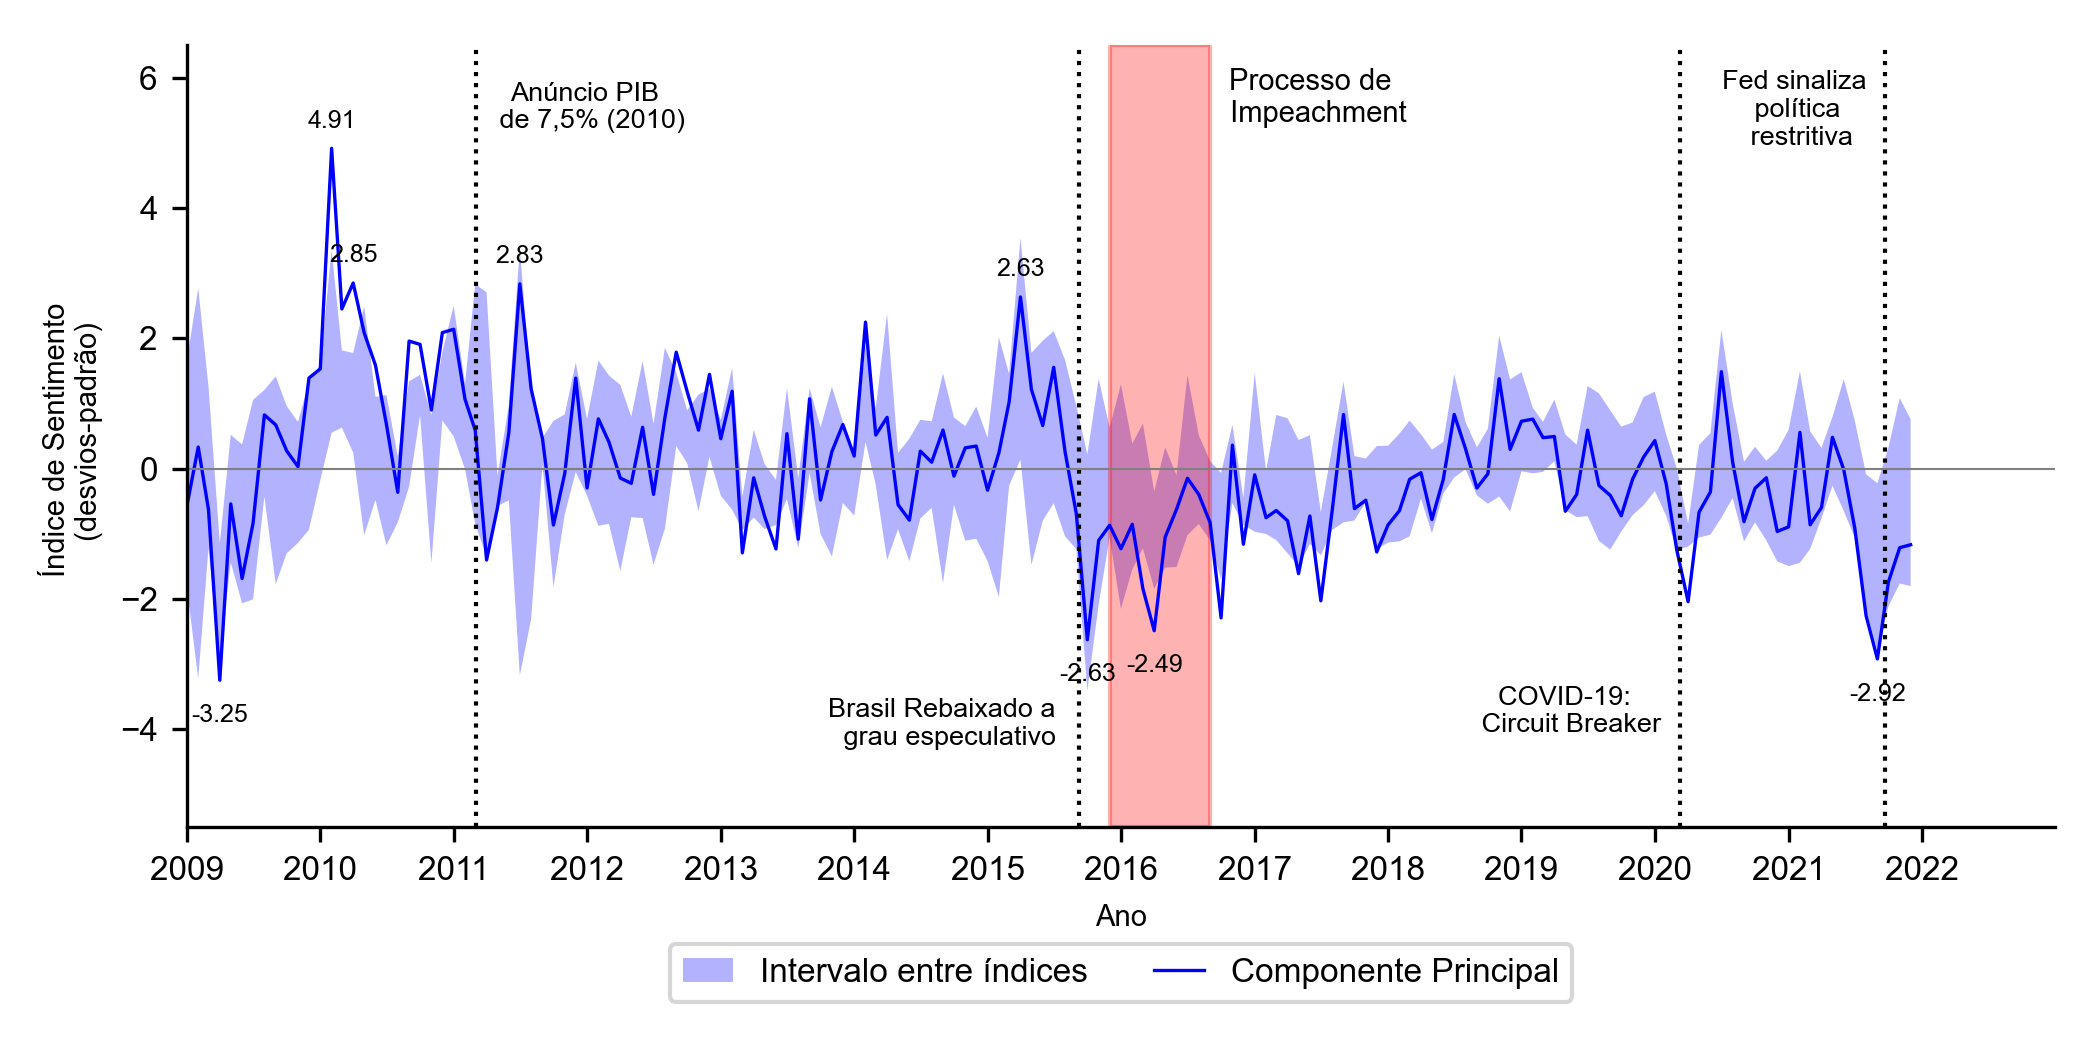
\includegraphics[width=\textwidth]{imagens/pca_plt.png} % Scales the image to fit within margins
    \label{graf:pca}
    \par\noindent
    \begin{minipage}{\textwidth}
        \centering
        \footnotesize % Adjust font size if needed
        \textit{Fonte: Elaboração Própria}
    \end{minipage}
\end{figure}

Da Figura \ref{graf:pca} é possível depreender a existência de dois regimes de comportamento do Componente Principal de forma que até 2016, os valores do índice de sentimento tendem a variar acima da média. Após esse período, a maior parte dos valores varia abaixo média. Além disso, os quatro picos com valores máximos estão localizados antes de 2016 e três picos com valores mínimos após esse ano. Se o valor do Componente Principal sintetiza a variação dos índices de sentimento, então é possível estender essa interpretação ao comportamento dos índices de forma individual.

É bem conhecida a deterioração do cenário político e econômico durante os anos de 2015 e 2016, onde o PIB caiu 3,5\% e 3,3\% respectivamente. Além disso, a inflação, mensurada pelo IPCA, atingiu 10,67\% em 2015, o maior valor da série desde 2002, forçando uma política monetária mais restritiva. 

De um modo geral, a evolução do Componente Principal dos índices de sentimento dialoga com importantes eventos econômicos e apresenta comportamento esperado durante certos intervalos. Esses resultados apontam para a utilização tanto dos índices particulares quanto do próprio componente principal que pode atuar como uma \textit{proxy} do comportamento de variação dos diversos índices. 

\clearpage

\section{Modelos}

Os modelos VAR e \textit{Local Projections} foram construídos segundo o ordenamento de variáveis proposto pela matriz \(B_0\), página \pageref{matrix:matriz_b_ordenamento}. Foram testados todos os oito índices de sentimento produzidos, bem como os dois componentes principais gerados a partir das duas fórmulas de agregação de sentimento. 

Para conferir robustez à modelagem foi aplicada uma ampla gama de variações em termos de transformação das variáveis, técnicas de estacionarização, escolha da ordem \(P\) de autoregressividade dos modelos, bem como foram promovidos novos ordenamentos na matriz \(B_0\) e mesmo inclusão ou exclusão de algumas variáveis. 

O melhor modelo obtido, levando em consideração como critério de julgamento a obtenção de significância estatística dos coeficientes estimados, foi aquele cujo índice de sentimento se fundamenta no dicionário SentiLex e na fórmula de agregação de \textcite{carosia_analyzing_2020}. As variáveis e o ordenamento da matriz \(B_0\) é exatamente o apresentado na seção \ref{metodologia_series_temporais}. As variáveis foram tomadas em nível com aplicação da transformação logarítmica seguindo o tratamento apresentado pela maior parte da literatura na Tabela \ref{tab:var_trabalhos_nacionais}. Adicionalmente, foi aplicado o filtro de sazonalidade X13-ARIMA-SEATS nas variáveis. A escolha da ordem do modelo foi realizada de acordo com o critério de informação AIC, que sugeriu a implementação de quatro \textit{lags} temporais. Todas as raízes do polinômio característico se encontram dentro do círculo unitário, confirmando a estabilidade do modelo. Inicialmente, todos as especificações foram construídas segundo o modelo VAR de forma a estabelecer uma conexão com a literatura nacional. Posteriormente, foram estendidas à modelagem \textit{Local Projections} de forma que pudessem ser geradas comparações entre as duas estratégias de modelagem. 

A Figura \ref{graf:lp_var_comparison} apresenta um comparativo das FRI geradas tanto pelo modelo VAR quanto pelo modelo \textit{Local Projections} segundo as especificações anteriormente definidas. As FRI representam as respostas dinâmicas de cada variável a um choque positivo de um desvio-padrão no termo de erro da variável de sentimento da política monetária. 

\begin{figure}[H]
    \captionsetup{position=above} % Coloca a legenda acima da imagem
    \caption{Funções de Impulso Resposta à um choque na variável de sentimento}
    \centering
    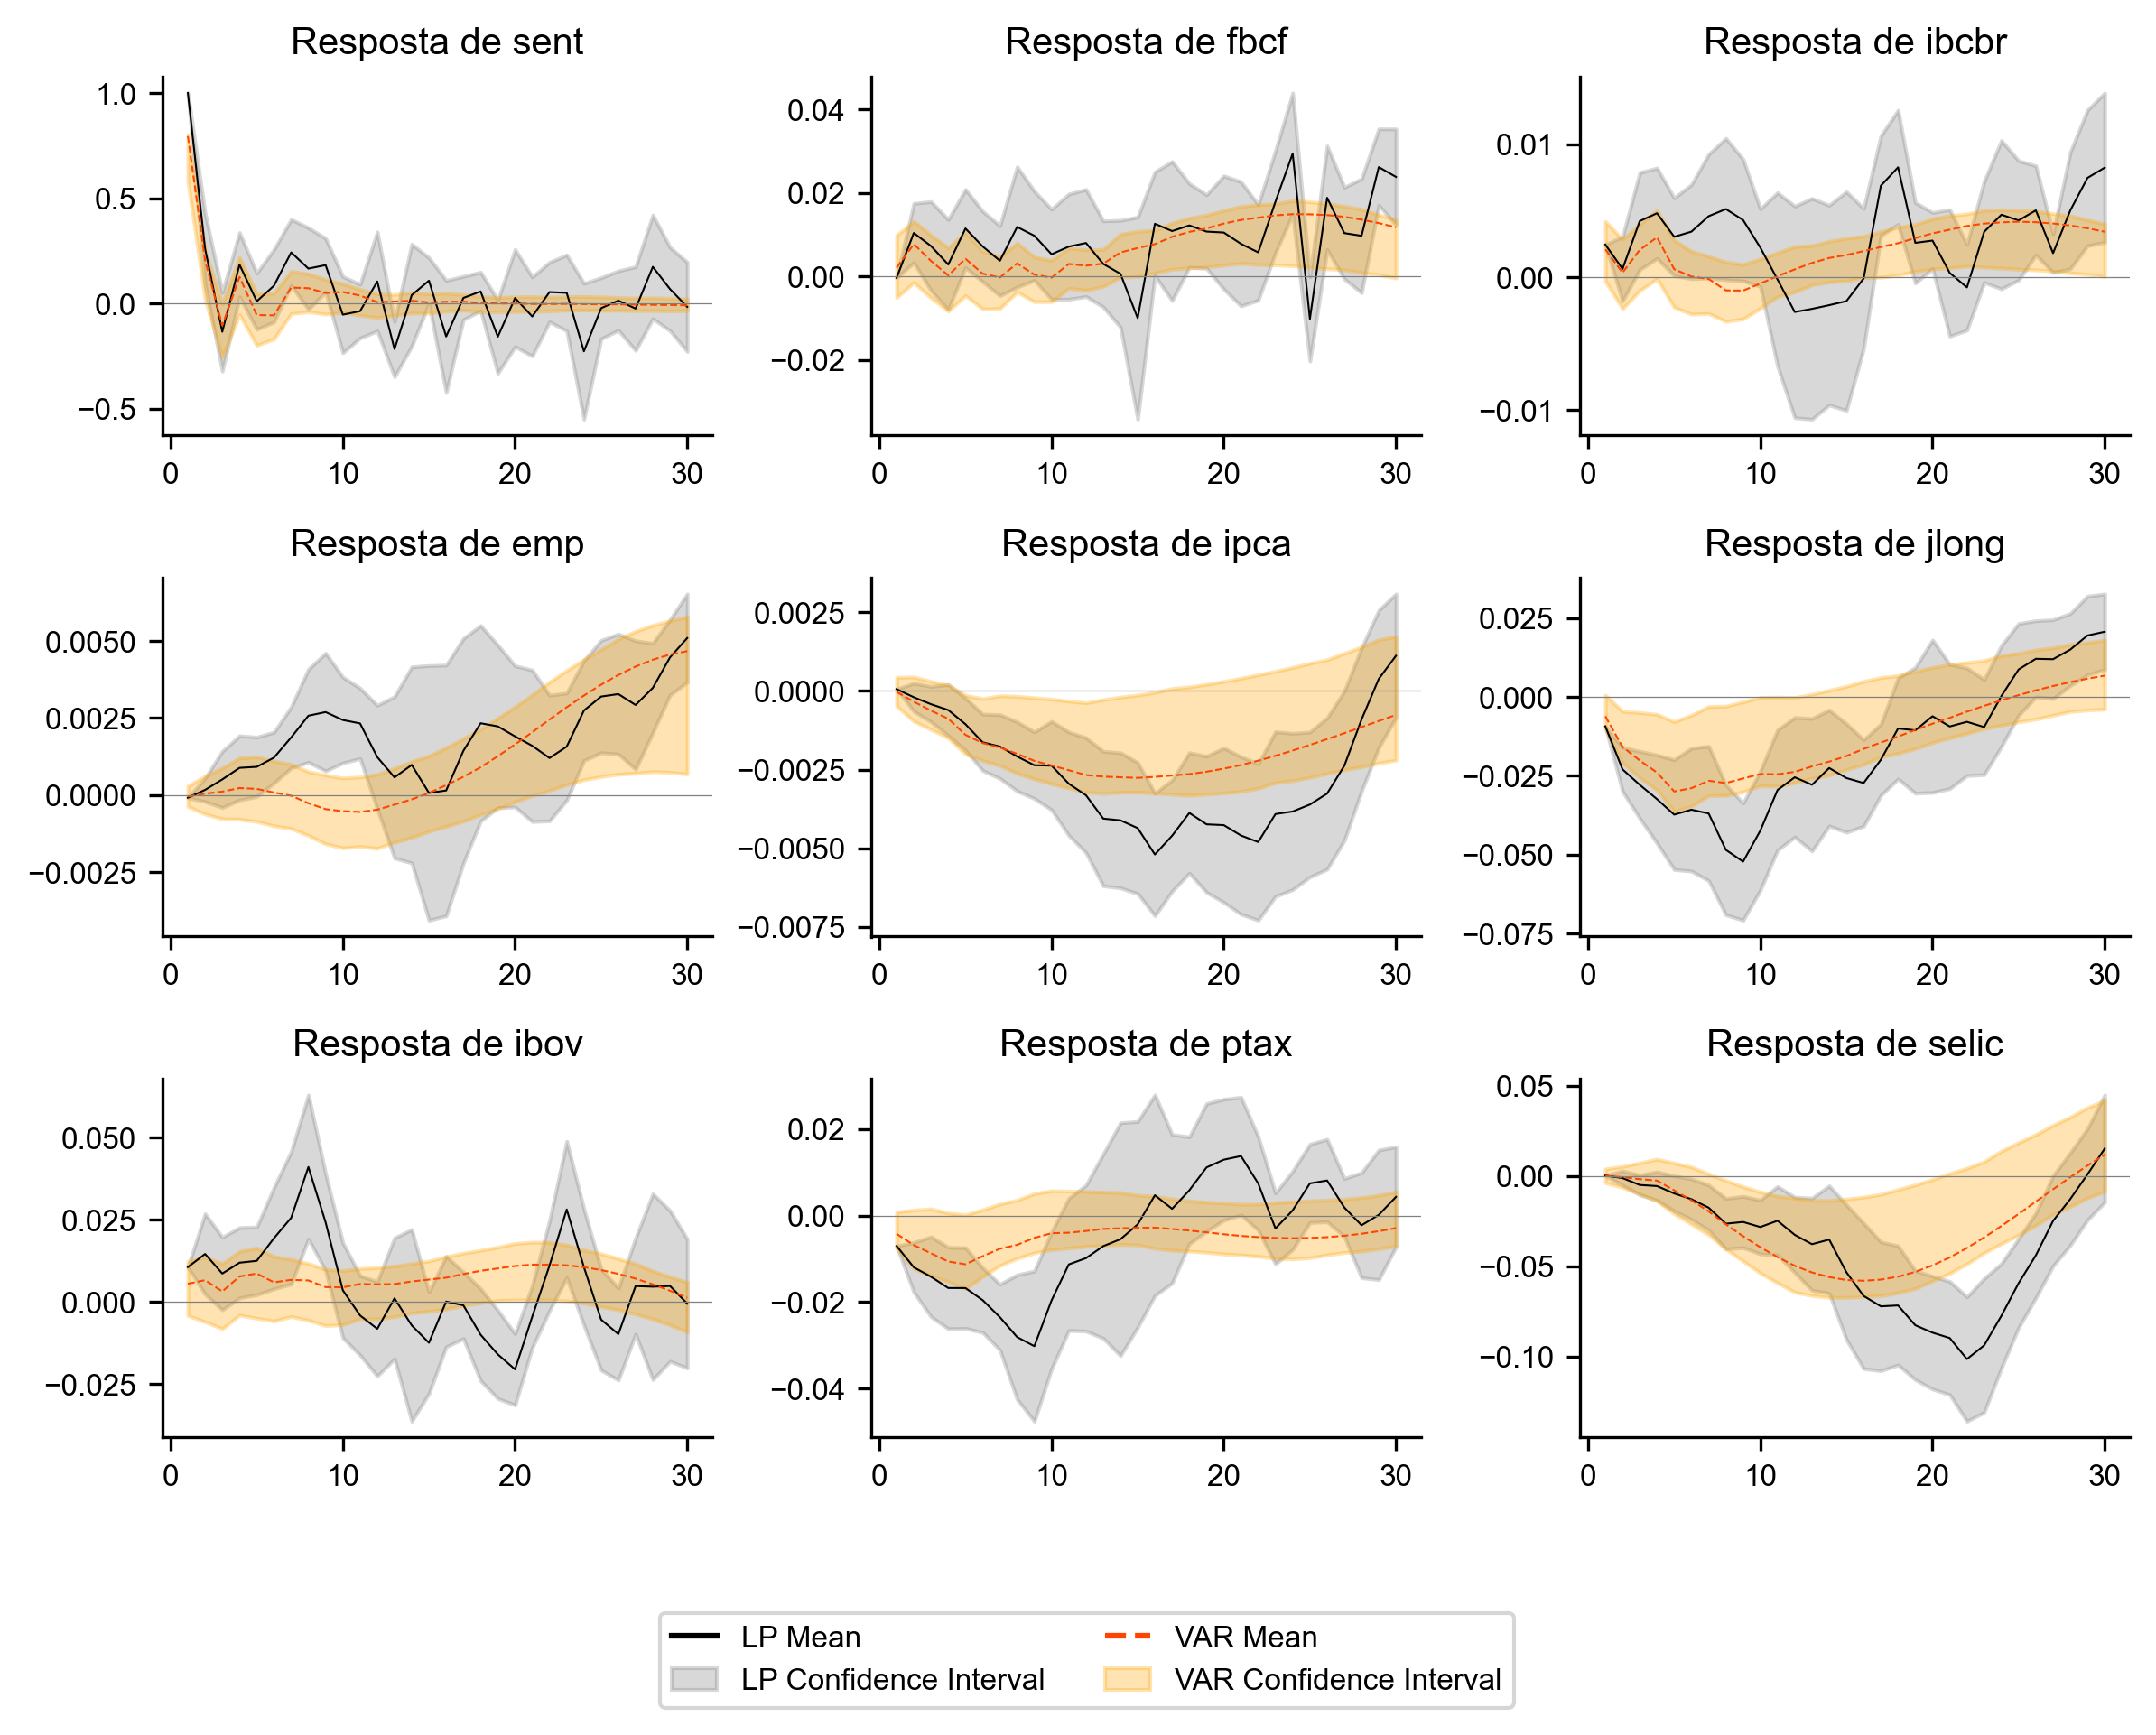
\includegraphics[width=\textwidth]{imagens/lp_var_comparison.png} % Adjust to fit within margins
    \label{graf:lp_var_comparison}
    \par\noindent
    \begin{minipage}{\textwidth}
        \centering
        \footnotesize % Adjust font size if needed
        \textit{Fonte: Elaboração Própria}
    \end{minipage}
\end{figure}

É possível depreender da Figura \ref{graf:lp_var_comparison} uma convergência entre os modelos VAR e \textit{Local Projections} no que se refere ao sentido do efeito das variáveis, especialmente as financeiras. Assim sendo, um choque positivo de um desvio-padrão na variável de sentimento da política monetária causa uma queda estatisticamente significante do IPCA entre quatro e quinze meses nos dois modelos. Essa queda se estende por um horizonte maior no modelo \textit{Local Projections} e com magnitude mais acentuada.

Uma resposta mais imediata ao choque positivo no sentimento ocorre com a variável de juros de longo prazo (jlong). Por ser uma variável tipicamente financeira, trata-se de um resultado esperado. Também para essa variável ambos os modelos apontam em um sentido comum do efeito: um choque positivo no sentimento diminui os juros de longo prazo com magnitude maior para o modelo de \textit{Local Projections} do que para o modelo VAR.

A Selic segue comportamento semelhante as taxas de juros de longo prazo, porém com efeito retardado. Trata-se de um resultado alinhado com a teoria, uma vez que a diminuição das taxas de juros de longo prazo reduz a inclinação da curva de juros, possibilitando margem de manobra para operação da taxa básica de juros. 

As outras duas variáveis financeiras, índice IBOVESPA (ibov) e o câmbio (ptax), apresentam resultados esperados e significativos para o modelo \textit{Local Projections}, mas não para o modelo VAR. Assim, um choque positivo na variável de sentimento da política monetária leva à uma valorização da bolsa de valores no primeiro caso e uma apreciação cambial no segundo. 

As variáveis reais apresentam um resultado mais intrigante. Tanto a FBCF, quanto o IBC-BR e o nível de emprego apresentam uma resposta positiva ao choque na variável de sentimento pelos dois modelos, contudo restritas a um prazo extenso. No modelo VAR, os coeficientes apenas são significativos após quinze ou vinte meses. O modelo \textit{Local Projections} apresenta significância em alguns intervalos antes desse período, mas não de forma consistente. Trata-se de um resultado que necessita de maior investigação para sua clareza, uma vez que pode indicar uma reação do setor real da economia a um choque positivo na política monetária \textit{ceteris paribus}, ou seja, já considerados os efeitos de variáveis financeiras importantes, tal como os juros de longo prazo. 





\bigskip

% Conserta o indent para alinhar conforme padrão de normalização
\addtocontents{toc}{\cftsetindents{chapter}{1.5cm}{3em}}
\addtocontents{toc}{\cftsetindents{section}{0cm}{1.5cm}}
\addtocontents{toc}{\cftsetindents{subsection}{0cm}{1.5cm}}
\addtocontents{toc}{\cftsetindents{subsubsection}{0cm}{1.5cm}}
\addtocontents{toc}{\protect\renewcommand{\protect\cftchapteraftersnum}{\enskip\textemdash\enskip}}


\printbibliography[title={REFERÊNCIAS}, heading=bibintoc] %

% ---
% Inicia os apêndices
% Para as seções nos apêndices usar o comando \section* que não adiciona a seção no sumário.
% ---
\appendix

\chapterstyle{apendices}

% ----------------------------------------------------------
\chapter{Derivação do Vetor de Médias}
% ----------------------------------------------------------


Seja o \(VAR(1)\) bivariado representado em sua forma reduzida:

\begin{equation}
X_t = A_0 + A_1X_{t-1} + e_t, 
\end{equation}

ou em notação matricial: 

\begin{equation}
\label{eq:var_reduz_matrix}
\begin{aligned} \begin{bmatrix}
z_t \\ y_t \end{bmatrix} &=\begin{bmatrix}
a_{10} \\ a_{20}\end{bmatrix} +
\begin{bmatrix}a_{11} & a_{12} \\a_{21} & a_{22}
\end{bmatrix}\begin{bmatrix} z_{t-1} \\ y_{t-1}
\end{bmatrix}  +\begin{bmatrix} e_{1t} \\ e_{2t}
\end{bmatrix}\end{aligned}
\end{equation}

Se

\begin{equation}
\left\{ 
\begin{array}{l}

\begin{bmatrix}e_{1t} \\e_{2t}
\end{bmatrix}\equiv B^{-1}\varepsilon_t =\begin{bmatrix}
\frac{\varepsilon_{zt} - b_{12} \varepsilon_{yt}}{1 - b_{12}b_{21}} \\[5pt]\frac{\varepsilon_{yt} - b_{21} \varepsilon_{zt}}{1 - b_{12}b_{21}}\end{bmatrix}
\\
\varepsilon_{zt} \sim \mathcal{RB}(0, \sigma^2_z) 

\end{array} 
\right.
\end{equation}

Então:
\begin{equation} \mathbb{E}(e_t) = \textbf{0} \end{equation}

Se, sob estacionariedade, para uma variável qualquer:

\begin{equation}
 \mathbb{E} \left( x_t \right) = \mathbb{E} \left( x_{t-1} \right) = \mu, \, \forall \, t \in \mathbb{Z} = \{0, \pm1, \pm2, ...\}
\end{equation}

Então, similarmente para \(z_t\) e \(y_t\), tem-se que os valores das séries flutuam em torno de suas médias de modo que \(\mathbb{E} \left( y_t \right) = \mathbb{E} \left( y_{t-1} \right) = \bar{y}\) e \(\mathbb{E} \left( z_t \right) = \mathbb{E} \left( z_{t-1} \right) = \bar{z}\).
 
Aplicando-se o operador de expectância sobre ambos os termos da equação \eqref{eq:var_reduz_matrix}, tem-se: 

\begin{equation}
\label{eq:expect_var}
\mathbb{E} \begin{bmatrix}z_t \\y_t\end{bmatrix} 
= 
\mathbb{E}\begin{bmatrix}a_{10} \\ a_{20}\end{bmatrix} 
+
\mathbb{E}\begin{bmatrix}
a_{11} & a_{12}\\a_{21} & a_{22}
\end{bmatrix}
\begin{bmatrix}z_{t-1} \\ y_{t-1}\end{bmatrix}
+
\mathbb{E}\begin{bmatrix}e_{1t} \\ e_{2t}\end{bmatrix}
\end{equation}

Uma vez que: 

\begin{equation}
\left\{ 
\begin{array}{l}
\mathbb{E} \begin{bmatrix}z_t \\y_t\end{bmatrix} 
= 
\begin{bmatrix}\mathbb{E}(y_t) \\\mathbb{E}(z_t)
\end{bmatrix} 
=
\begin{bmatrix}\bar{y} \\\bar{z}\end{bmatrix}
\\[15pt]
\mathbb{E} \begin{bmatrix}a_{10} \\a_{20}\end{bmatrix}
=
\begin{bmatrix}a_{10} \\a_{20}\end{bmatrix}
\\[15pt]
\mathbb{E}\begin{bmatrix}
a_{11} & a_{12}\\a_{21} & a_{22}\end{bmatrix}
\begin{bmatrix}z_{t-1} \\ y_{t-1}\end{bmatrix}
=
\begin{bmatrix}
a_{11} & a_{12}\\a_{21} & a_{22}\end{bmatrix}
\mathbb{E}\begin{bmatrix}z_{t-1} \\ y_{t-1}\end{bmatrix}
\\[15pt]
=
\begin{bmatrix}
a_{11} & a_{12}\\a_{21} & a_{22}\end{bmatrix}
\begin{bmatrix} \mathbb{E}(z_{t-1})
\\ \mathbb{E}(y_{t-1})\end{bmatrix}
~~ = 
\begin{bmatrix}
a_{11} & a_{12}\\a_{21} & a_{22}\end{bmatrix}
\begin{bmatrix}\bar{y} \\\bar{z}\end{bmatrix}
\end{array} 
\right.
\end{equation}

Então a equação  \eqref{eq:expect_var} pode ser reescrita da seguinte maneira:

\begin{equation}
\begin{bmatrix}
\bar{z} \\\bar{y}
\end{bmatrix}=
\begin{bmatrix}a_{10} \\a_{20}\end{bmatrix}
+\begin{bmatrix}a_{11} & a_{12} \\ a_{21} & a_{22}
\end{bmatrix}\begin{bmatrix}\bar{z} \\\bar{y}
\end{bmatrix}\end{equation}

De onde os valores de longo prazo da série podem ser encontrados mediante resolução do sistema linear:

\begin{equation}\begin{bmatrix}
\bar{z} \\\bar{y}
\end{bmatrix}-\begin{bmatrix}
a_{11} & a_{12} \\a_{21} & a_{22}
\end{bmatrix}\begin{bmatrix}\bar{z} \\\bar{y}
\end{bmatrix}=\begin{bmatrix}a_{10} \\a_{20}
\end{bmatrix}\end{equation}

\begin{equation}\left(\begin{bmatrix}1 & 0 \\0 & 1
\end{bmatrix}-\begin{bmatrix}
a_{11} & a_{12} \\a_{21} & a_{22}
\end{bmatrix}\right)\begin{bmatrix}
\bar{z} \\\bar{y}\end{bmatrix}
=\begin{bmatrix}a_{10} \\a_{20}
\end{bmatrix}\end{equation}

\begin{equation}
\underbrace{
\begin{bmatrix}\bar{z} \\\bar{y}
\end{bmatrix}
}_{\equiv \bar{X}}
=
\left(
\underbrace{
\begin{bmatrix}1 & 0 \\0 & 1\end{bmatrix}
}_{\equiv I}
-
\underbrace{
\begin{bmatrix}a_{11} & a_{12} 
\\a_{21} & a_{22}\end{bmatrix}
}_{\equiv A_1}
\right)^{-1}
\underbrace{
\begin{bmatrix}a_{10} \\a_{20}\end{bmatrix}
}_{\equiv A_0}
\end{equation}

% ----------------------------------------------------------
% \chapter{Visualizações das pilhas de areia}\label{caleidoscopios}
% % ----------------------------------------------------------
% \lipsum[10]


% \section*{Visualização da característica fractal da pilha de areia}
% \lipsum[10]

% ---
% Inicia os anexos
% ---
\addtocontents{toc}{\protect\renewcommand\protect\cftappendixname{\nomeanexo~}}
\appendix
\chapterstyle{anexos}

% Imprime uma página indicando o início dos apêndices





% % ----------------------------------------------------------
% \chapter{Anexos}
% % ----------------------------------------------------------
% \lipsum[5]

% % ----------------------------------------------------------
% \chapter{outro anexos}

% \lipsum[5]

% \section*{seção no anexo}

% \lipsum[5]

% \section*{Outra seção no anexo}

% \lipsum[5]





\end{document}